\begin{refsection}

\hypertarget{from-local-seafloor-imagery-to-global-patterns-in-benthic-habitats-contribution-of-citizen-science-to-habitat-classification-across-latitudes}{%
\chapter{From local seafloor imagery to global patterns in benthic
habitats: contribution of citizen science to habitat classification
across
latitudes}\label{from-local-seafloor-imagery-to-global-patterns-in-benthic-habitats-contribution-of-citizen-science-to-habitat-classification-across-latitudes}}

\hypertarget{preambule-chapter2}{%
\section*{Préambule}\label{preambule-chapter2}}
\addcontentsline{toc}{section}{Préambule}

Le Chapitre 1 a permis de mettre en évidence deux limites majeures de
l'application des \emph{jSDM} (\emph{Joint Species Distribution Models})
pour comprendre la structure des communautés et le rôle sous-jacent des
habitats. Premièrement, que ce soit sur des données de présence/absence
ou bien d'abondance, le framework de \emph{jSDM} testé ici présentait
des performances de prédiction de la biodiversité faible, limitant
grandement ses capacités d'extrapolation spatiales et/ou temporelles.
Deuxièmement, le \emph{jSDM} étudié dans le chapitre précédent
nécessitait une importante puissance de calcul pour ajuster aux 99
espèces les plus de 16 000 paramètres nécessaires tout en leur assurant
une convergence suffisante des estimations de paramètres. Ainsi, son
application sur un jeu de données plus conséquent du \emph{Reef Life
Survey}, avec une communauté faunistique de plus de 3 000 taxons, nous a
semblé limiter son potentiel pour analyser un tel jeu de données à
l'échelle globale. De plus, dans un projet antérieur focalisé sur
l'usage des \emph{jSDM} pour l'inférence de réseau de co-occurrence des
espèces benthiques \autocite{Violet_2020}, nous avons fait face à des
incertitudes méthodologiques pour caractériser de manière robuste les
réseaux d'interactions potentiels. En effet, les réseaux reconstitués
avaient été soumis aux jugements d'un panel d'experts benthologues dont
les avis discordants n'ont pas permis de valider la véracité des
interactions identifiées. C'est pourquoi pour mieux comprendre comment
les habitats biogéniques structurent les communautés associées à
l'échelle mondiale, nous avons changé de stratégie et nous avons adopté
la méthode ``\emph{agréger, puis prédire}'' suggérée par
\textcite{Ferrier_2006}. L'objet central de ce chapitre réside dans
l'application d'une méthode de groupement peu appliquée en écologie afin
d'identifier différents états d'habitats. Le chapitre 3 complètera cette
partie d'agrégation des données par une partie prédictive.

Les particularités des données écologiques et notamment celles issues de
sciences participatives (hétérogénéité, bruit dans les données,
relations non-linéaires entre les variables d'un écosystème, etc.)
limitent la pertinence de certaines méthodes de groupement (p.~ex.
k-means, classification hiérarchique à lien simple complet, ou selon la
méthode de Ward) classiquement utilisées en écologie
(Fig.~\ref{fig:chap2chapo1}). Nous avons utilisé dans ce chapitre une
nouvelle approche de groupement pour (1) distinguer différents états
d'habitats biogéniques à partir de données issues des sciences
participatives (2) identifier des habitats iconiques, et (3)
éventuellement détecter des transitions entre différents types
d'habitats. Ce chapitre a également pour but d'étudier la distribution
de ces états d'habitats à l'échelle du globe pour valider ou non les
groupes iconiques identifiés.

\begin{figure}
\hypertarget{fig:chap2chapo1}{%
\centering
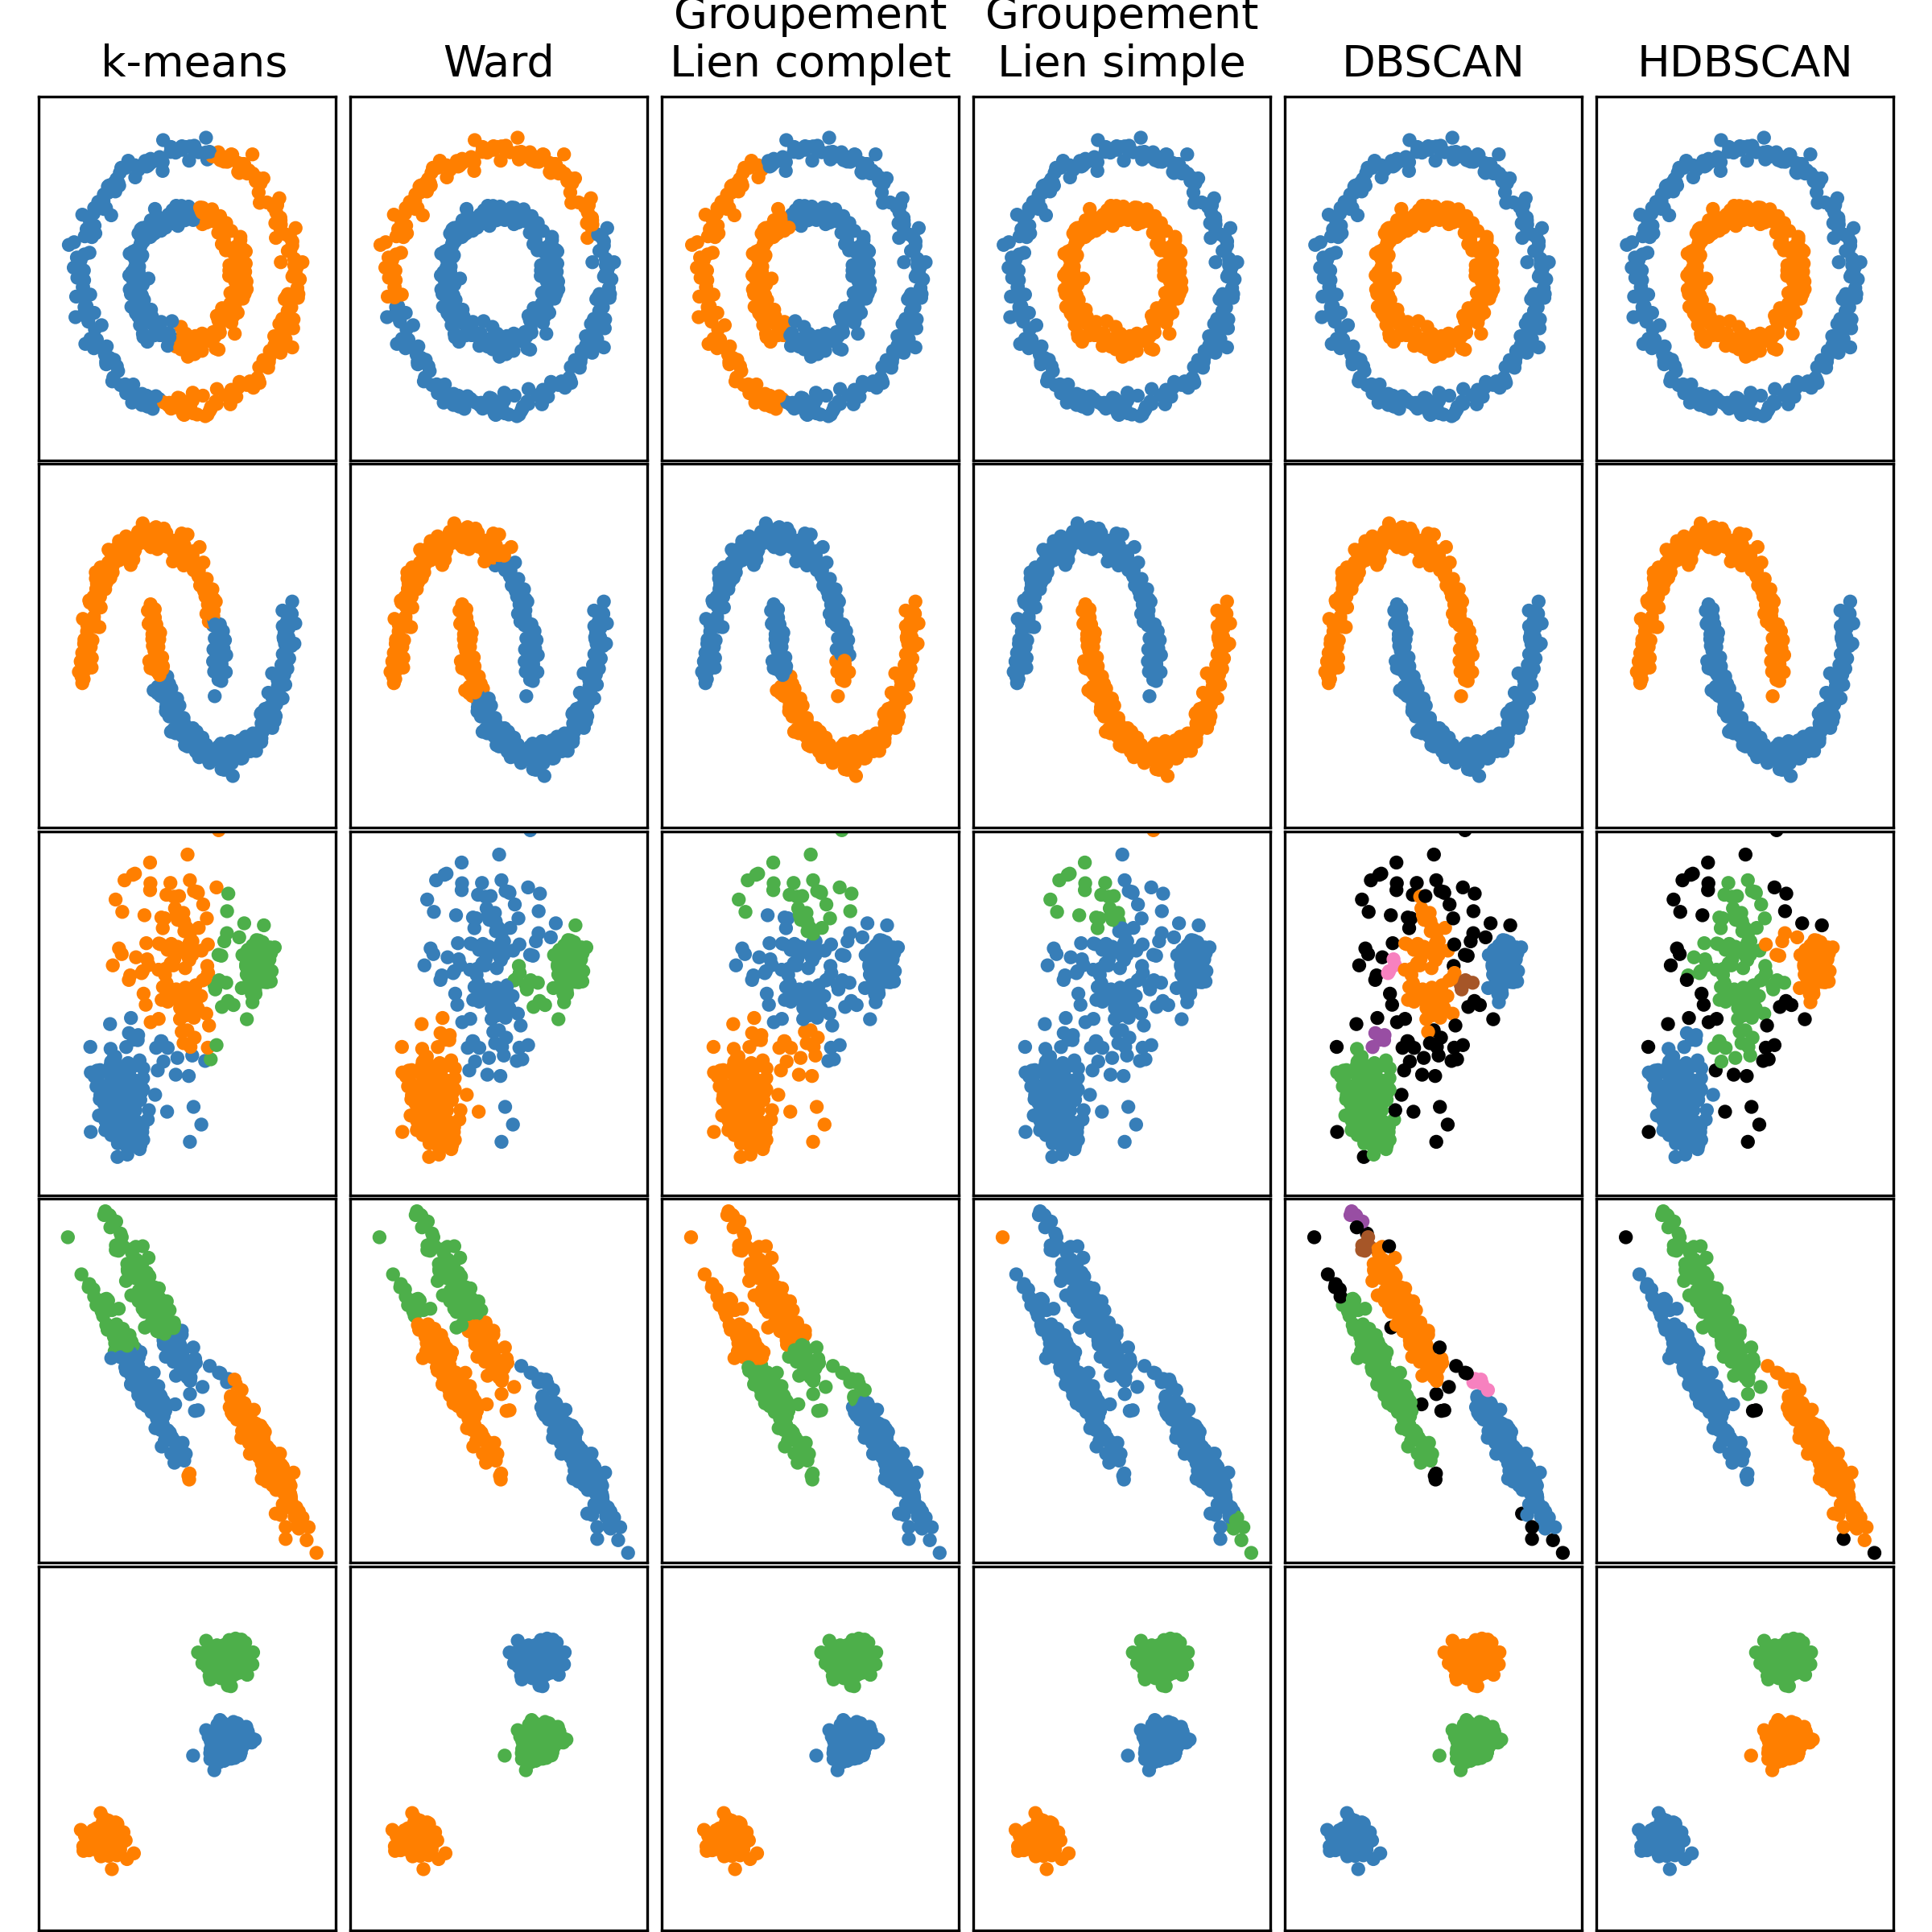
\includegraphics{03-Chapitre2/figures/synthetic_clustering_perf.png}
\caption[Comparaison de différents algorithmes de groupement utilisés en
écologie.]{Comparaison de différents algorithmes de groupement utilisés en
écologie (en colonne; à savoir k-means, Ward, groupement lien complet ou
lien simple, \mbox{DBSCAN} ou \mbox{HDBSCAN}) sur différents jeux de données simulés
en deux dimensions (en ligne). Les jeux de données des deux premières
lignes contiennent deux groupes, les trois derniers en contiennent
trois.}\label{fig:chap2chapo1}
}
\end{figure}

En amont de ce chapitre, j'ai étudié le comportement de plusieurs
combinaisons de méthodes de réductions de dimensions, ainsi que de
groupement (Fig.~\ref{fig:chap2chapo1}) ce qui a orienté le choix pour
ce Chapitre 2 vers une méthodologie qui combine un algorithme de
réduction basé sur le principe des graphes de voisinage (\emph{UMAP};
\textcite{McInnes_2020}), et une méthode de groupement basée sur la
densité (\emph{HDBSCAN}; \textcite{Moulavi_2014} ;
\textcite{McInnes2017}). En appliquant cette méthode à des données
estimant le pourcentage de couverture de différents habitats sur la base
des photoquadrats obtenus sur plus de 6 500 transects réalisés en
plongée par des volontaires du programme \emph{Reef Life Survey}, nous
avons identifié 17 états d'habitats. Certains de ces habitats
représentent des états d'habitats benthiques iconiques comme les forêts
de laminaires ou des herbiers marins, alors que d'autres représentent
des états d'habitats considérés comme dégradés, par exemple les états
dominés par la présence d'algues gazonnantes.

Ce chapitre de thèse est l'oeuvre de la collaboration de Clément Violet, Aurélien Boyé, Graham Edgar, Elizabeth Oh, Rick Stuart-Smith et de Martin Marzloff. Ce chapitre a déjà fait l'objet d'une communication orale
``\emph{Predicting reef state and regime shift risk using machine
learning and the Reef Life Surve}y'' au 13th International Temperate
Reefs Symposium 2023. Ce chapitre devrait être prochainement proposé
pour publication au journal \emph{Global Ecology and Biogeography}.

\clearpage

\hypertarget{abstract-chapt2}{%
\section{Abstract}\label{abstract-chapt2}}

\textbf{Aim:} The aim of this study was to define reef benthic habitat
states and explore their spatial and temporal variability at a global
scale using an innovative clustering pipeline.

\textbf{Location:} The study uses data on the transects surveyed on
shallow (\(<~20\)m) reef ecosystems across the globe.

\textbf{Time period:} Transects sampled between 2008 and 2021.

\textbf{Major taxa studied:} Macroalgae, sessile invertebrates,
hydrozoans, seagrass, corals.

\textbf{Methods:} Percentage cover was estimated for 24 functional
groups of sessile biota and substratum from annotated underwater
photoquadrats taken along 6,554 transects by scuba divers contributing
to the \emph{Reef Life Survey} dataset. A clustering pipeline combining
a dimension-reduction technique, \emph{Uniform Manifold Approximation
and Projection} (\emph{UMAP}), with \emph{Hierarchical Density-Based
Spatial Clustering of Applications with Noise} (\emph{HDBSCAN}), was
used to identify benthic habitat states. Spatial and temporal variation
in habitat distribution was then explored across ecoregions.

\textbf{Results:} The \emph{UMAP-HDBSCAN} pipeline identified 17
distinct clusters representing different benthic habitats and gradients
of ecological state. Certain habitat states displayed clear
biogeographic patterns, predominantly occurring in temperate regions or
tropical waters. Notably, some reefs dominated by turf algae, were
ubiquitous regardless of latitudes. Transition zones between temperate
and tropical waters emerged as spatial hotspots of habitat state
diversity. Temporal patterns revealed, changes in the proportion of
certain states showing variations over time, notably an increase in turf
algae occurrence.

\textbf{Main Conclusions:} The \emph{UMAP-HDBSCAN} clustering pipeline
effectively characterised fine-scale benthic habitat states at a global
scale, confirming known broader biogeographic patterns, including the
importance of temperate-tropical transition zones as hotspots of habitat
state diversity. This fine-scale, yet broadly-scalable habitat
classification could be applied as a standardised template for tracking
benthic habitat change across space and time at a global scale. The
\emph{UMAP-HDBSCAN} pipeline has proven to be a powerful and versatile
approach for analysing complex biological datasets and can be applied in
various ecological domains.

\clearpage

\hypertarget{intro-chapt2}{%
\section{Introduction}\label{intro-chapt2}}

Benthic habitats contribute to marine coastal ecosystems functioning and
the services they provide \autocite{Barbier_2011}. More specifically,
they contribute to shoreline protections \autocite{Barbier_2017}, carbon
sequestration \autocite{Fourqurean_2012}, support commercial fisheries
\autocite{Barbier_2017} and host diverse species and communities
\autocite{Sunday_2017}. As modifiers to abiotic substrates, foundation
species, such as kelp, seagrass, and corals engineer biogenic habitats
that contribute to specific functions of coastal ecosystems
\autocite{Elith_2009}. For instance, the tridimensional structure of
coral reefs can shelter fish assemblages from predators
\autocite{Hixon_1993}; seaweed or mussel beds can buffer environmental
conditions \autocites[ ]{Jurgens_2022}{Whitaker_2023}; and kelp forests
are both habitat and food sources for various fish and invertebrate
species \autocite{Edgar_2004}. Thus, changes in coastal benthic habitats
have direct cascading consequences on marine ecosystem structure,
functioning and services.

Being hotspots of human activity, coastal ecosystems can be adversely
affected by multiple anthropogenic stressors \autocites[
]{Bowler_2020}{Halpern_2019}. Global climate change can also lead to
fast changes in coastal abiotic conditions \autocites[
]{Burrows_2014}{Bowler_2020}. The impact of these multiple stressors on
benthic communities and ecosystems are mostly mediated by the response
of biogenic habitats like kelp, seagrass, or coral \autocites[
]{Harley_2006}{Rocha_2015b}. For example, in the vicinity of urban
areas, eutrophication can induce the replacement of kelp forests by turf
algae \autocites[ ]{Filbee-Dexter_2018}{Pessarrodona_2021}, marine
heatwaves can lead to coral bleaching, and their intensification in
magnitude and frequency can induce long-term decline in tropical coral
reefs \autocite{Bellwood_2004}, and overfishing of herbivorous fish in
these reefs can lead to the overgrowth of macroalgae on top of coral
reefs \autocite{Hughes_2007}. Hence, habitat changes are amongst the
greatest symptoms of anthropogenic impacts on shallow marine systems,
with large consequences for marine biodiversity \autocite{Rocha_2015a}.
As anthropogenic stressors on marine ecosystems tend to increase and
diversify \autocite{Halpern_2019}, habitat changes will likely become
more frequent in the future at a global scale \autocite{Conversi_2015}.
Yet, both the drivers of habitat change and its consequence on
biodiversity remain largely understudied in marine ecosystems
\autocite{Mazor_2018}.

Detecting and anticipating future habitat changes in benthic ecosystems
requires a thorough understanding of the current state and distribution
of benthic habitats and characterising of underlying drivers across
multiple scales. Currently, detailed knowledge of habitat distribution
is mostly local, i.e.~at scales ranging from study sites (10 m - 100 m)
or bay (100 m - 10 km) up to regions (10 km - 100 km) (e.g.
\textcite{Robert_2015} ; \textcite{Wicaksono_2019}), for instance using
remote sensing, acoustic surveys, or rather local monitoring of abiotic
conditions and communities \autocite{Costello_2009}. At larger scales,
habitat distribution maps are largely based on physical,
geomorphological and biogeochemical ocean properties (e.g.
\textcite{Brown_2011} ; \textcite{Lecours_2015} ;
\textcite{Sonnewald_2020}). At such scales, habitat maps either
disregard biogenic habitats or remain species-specific. Indeed, studies
that focus on biogenic habitat distribution tend to consider specific
habitat-formers independently \autocites[ ]{Assis_2020}{McKenzie_2020}
and rarely provide information on community composition. Large-scale
seafloor habitat maps of either abiotic, or biogenic features also tend
to integrate data over large timescales (e.g.~decades). Their aim is
rather to provide a static picture of the potential distribution of
these habitats than to infer changes in habitat states and distribution.
Knowledge of benthic habitat changes thus remains highly regional (e.g.
\textcite{Cattano_2020}). In that context several global studies have
collated heterogeneous regional monitoring data to document changes in
emblematic habitat-formers, such as seagrass spp. \autocites[
]{Waycott_2009}{Dunic_2021}, kelp beds \autocites[
]{Krumhansl_2016}{Filbee-Dexter_2018} or coral reefs
\autocite{Eddy_2021}. Yet, these independent studies on specific
habitat-formers are not sufficient to gain a comprehensive understanding
of how the seafloor habitat mosaic has changed over the last decade at a
global scale and how it is now changing in the face of anthropogenic
pressures. Our understanding of current changes in seafloor habitat
mosaic is impeded by the lack of large-scale, standardised, data-driven
definition and maps of benthic habitat and their potential states.

Identifying changes in benthic habitat states through space and time
requires a standardised workflow from data collection through to
systematic statistical discrimination between habitat states. In this
study, we aim to develop a data-driven pipeline that distinguishes
different iconic benthic habitats observed spatially, and apply this to
characterise stepwise changes in habitat ecological states through time.
Because scientific monitoring programmes are often expensive
\autocite{Edgar_2016} and restricted in their spatial and/or temporal
coverage \autocite{Rhodes_2015}, participatory science programmes have
emerged as valuable means to increase monitoring programme coverage and
resolution. In this study, we leverage the benefits of a citizen science
program to characterise benthic habitat states at the global scale and
overcome the limitations of traditional scientific programs. The
\emph{Reef Life Survey} (\emph{RLS}) relies on standardised diver-based
50-metre-long transects to estimate fish and invertebrate species
abundance as well as image-based percentage cover of coastal benthic
habitats \autocite{Edgar_2014b}. Estimates of habitat percentage cover
have already proven useful for defining habitat states at a regional
scale through the use of unsupervised machine learning techniques
\autocites[ ]{Cresswell_2017}{PelletierD_2020}. However, the methods
proposed in these previous studies come with a number of limitations
when upscaling these approaches at a global scale. In particular, the
occurrence and abundance of habitat-forming species are expected to show
non-linear responses to environmental changes \autocite{Oksanen_2002},
especially across large environmental gradients. Still, the clustering
algorithm used for \textcite{Cresswell_2017} and
\textcite{PelletierD_2020} are not adapted to take into account the
non-linear nature of the dominance patterns between different
habitat-forming species.

Hence, we applied a new workflow, combining two algorithms to overcome
these challenges: (1) \emph{Uniform Manifold Approximation and
Projection} (\emph{UMAP}) a novel dimension reduction technique
preserving complex nonlinear structures and patterns
\autocite{McInnes_2020}, (2) and the \emph{Hierarchical Density-Based
Spatial Clustering of Applications with Noise algorithm}
(\emph{HDBSCAN}) that can identify clusters of varying shapes and sizes
while filtering out outlier noise \autocites[
]{Campello_2013}{McInnes2017}. While previous ecological studies have
successfully applied both \emph{UMAP} for dimension reduction
\autocite{Milosevic_2022} and \emph{HDBSCAN} for food web classification
\autocite{Ohlsson_2020}, our study represents a novel application to
coastal marine habitats. We interpret classification results by
combining the latest \emph{SHapley Additive exPlanations} (\emph{SHAP})
\autocite{Lundberg_2017} framework with visual inspections of
photoquadrats associated with the most representative transects of the
different clusters.

Therefore, the aim of this study is to characterise coastal benthic
habitat states using a \emph{UMAP-HDBSCAN} pipeline on the \emph{RLS}
habitat dataset. Using this pipeline, we identify and classify benthic
habitat states at a global scale and characterise their spatial and
temporal variability across biogeographical gradients as well as within
bioregions.

\clearpage

\hypertarget{mat-met-chapt2}{%
\section{Materials \& Methods}\label{mat-met-chapt2}}

We used a \emph{UMAP-HDBSCAN} pipeline to cluster the global \emph{RLS}
benthic habitat dataset. In the following sections, we sequentially
describe : (1) the data used in this study, (2) the clustering pipeline,
(3) the interpretation of the identified clusters.

\hypertarget{data}{%
\subsection{Data}\label{data}}

\hypertarget{reef-life-survey-photoquadrat-dataset}{%
\subsection{\texorpdfstring{\emph{Reef Life Survey} photoquadrat
dataset}{Reef Life Survey photoquadrat dataset}}\label{reef-life-survey-photoquadrat-dataset}}

The \emph{RLS} (\url{http://www.reeflifesurvey.com/}) is a hybrid
citizen science/professional researcher program monitoring reef
communities around the world using scuba-diving visual census. Details
about the survey methods, including protocols, diver training, data
quality assurance and data management, are covered by
\textcite{Edgar_2014}. Here, we used estimates of relative cover of
benthic habitats derived from in situ digital photoquadrats: along
standardised 50 m transect, 20 photoquadrats, which each approximately
covers 0.3 m × 0.3 m, are collected every 2.5 m \autocite{Edgar_2020}.
Images are then annotated using point counts on the \emph{Squidle+}
(\url{https://squidle.org/}) platform to estimate the percentage covers
of about 50 substratum types and functional groups, based on the
\emph{CATAMI} benthic imagery classification scheme
(\textcite{Althaus_2015} ; for further details, see
\textcite{Edgar_2020}). Based on \emph{RLS} specialists' expertise,
these 50 original benthic habitat categories (see Appendix A, Table 1 in
Supporting Informations) were grouped into 24 broader categories
(Table~\ref{tbl:chap2table1}) that more consistently capture the range
of dominant coastal substratum available along \emph{RLS} transects at
the global scale.

We extracted the \emph{RLS} photoquadrat dataset on 24 January 2023.
From the original 8,154 transects, we removed partially scored
transects. For transects annotated multiple times on \emph{Squidle+}
across various research projects, mean percentage cover estimates were
considered. After fully curating the dataset, the photoquadrat dataset
consisted of 6,554 transects across 2,249 sites over the world. All
subsequent analyses were performed at the transect level to consider
local-scale variation in the state of benthic habitats.

\hypertarget{tbl:chap2table1}{}
\begin{longtable}[]{@{}
  >{\centering\arraybackslash}p{(\columnwidth - 2\tabcolsep) * \real{0.2614}}
  >{\raggedright\arraybackslash}p{(\columnwidth - 2\tabcolsep) * \real{0.7386}}@{}}
\caption[Description of the 24 categories used in
this study to overall capture the diversity of habitat types sampled by
\emph{Reef Life Surveys} worldwide.]{\label{tbl:chap2table1}Description of the 24 categories used in
this study to overall capture the diversity of habitat types sampled by
\emph{Reef Life Surveys} worldwide. The 50 original \emph{RLS}
categories were lumped into these 24 categories that represent
ecologically-consistent groups associated with different levels of
structural complexity.}\tabularnewline
\toprule\noalign{}
\begin{minipage}[b]{\linewidth}\centering
\textbf{Habitat Categories}
\end{minipage} & \begin{minipage}[b]{\linewidth}\raggedright
\textbf{Description}
\end{minipage} \\
\midrule\noalign{}
\endfirsthead
\toprule\noalign{}
\begin{minipage}[b]{\linewidth}\centering
\textbf{Habitat Categories}
\end{minipage} & \begin{minipage}[b]{\linewidth}\raggedright
\textbf{Description}
\end{minipage} \\
\midrule\noalign{}
\endhead
\bottomrule\noalign{}
\endlastfoot
\multicolumn{2}{@{}c@{}}{%
\emph{Erect algae}}\\\hline

Large canopy forming algae & Large overstorey algae forming a canopy,
including kelps or large fucoids \\
Bushy Fucoid like & Robust vertical leaf-liked shaped brown algae \\
Other Brown algae & Thick or thin-sheet like vertical algae \\
Red algae & Foliose vertical red algae \\
Green algae & Thin-sheet like, thick, or ribbon-like, vertical growth
algae \\\hline
\multicolumn{2}{@{}c@{}}{%
\emph{Erect calcareous algae}} \\\hline
Geniculate coralline algae & Red vertical calcified segmented algae \\
Green calcified algae & Small calcified green algae \\
\hline
\multicolumn{2}{@{}c@{}}{%
\emph{Encrusting algae}} \\\hline
Crustose coralline algae & Red algae forming a small calcified crust
over hard substrate \\
Encrusting algae & ~Algae forming a leathery crust over a substrate \\
\hline
\multicolumn{2}{@{}c@{}}{%
\emph{Mat-forming Algae}} \\\hline
Filamentous algae & Filamentous algae, epiphyte or rock-attached \\
Turf algae & Fine and mat-forming filamentous algae growing on hard
substrate \\
\hline
\multicolumn{2}{@{}c@{}}{%
\emph{Plant}} \\\hline
Seagrass & Vertical ribbon-like marine plant \\
\hline
\multicolumn{2}{@{}c@{}}{%
\emph{Sessile invertebrates}} \\\hline
Encrusting corals & Stony corals forming a crust over hard substrate \\
Branching coral & Branching coral forming large colonies \\
Foliose/Plate corals & Stony corals forming tabular or foliaceous
colonies \\
Massive corals & Stony corals characterised by large, ball- or
boulder-shaped colonies with a compact structure \\
Large-polyp stony corals & Large lobed stony coral, usually
free-living \\
Soft corals and gorgonians & Soft coral or gorgonian in the sub-class
Octocorallia \\
Calcareous hydrocorals and octocorals & Branching or foliaceous
coral-like \\
Other sessile invertebrates & Habitat-forming sessile invertebrates
(e.g.~sponges, ascidians, bryozoans or molluscs) excluding corals \\
\hline
\multicolumn{2}{@{}c@{}}{%
\emph{Seabed Materials}} \\
\hline
Dead coral & Dead attached coral skeleton \\
Bare rocky substrate & Bare rock \\
Unconsolidated substrate & Gravel, shell, coral rubble \\
Sand & Sand and fine sediments \\
\end{longtable}

\clearpage

\hypertarget{clustering-pipeline}{%
\section{Clustering pipeline}\label{clustering-pipeline}}

To account for non-linear, high-dimensional and complex nature of the
ecological data, we combined a graph theoretical dimension reduction
technique and a density-based classification technique, which has
successfully identified ecoprovinces using biogeochemical ocean data at
a global scale \autocite{Sonnewald_2020}. Among the set of methods
available, we have chosen the \emph{UMAP} algorithm
\autocite{McInnes_2020} and the \emph{HDBSCAN} algorithm \autocites[
]{Campello_2013}{McInnes2017} for dimension reduction and clustering,
respectively.

\hypertarget{dimension-reduction---umap}{%
\subsection{\texorpdfstring{Dimension reduction -
\emph{UMAP}}{Dimension reduction - UMAP}}\label{dimension-reduction---umap}}

The \emph{UMAP} algorithm is a non-linear reduction technique
\autocite{McInnes_2020}. Unlike more traditional methods applied in
ecology such as \emph{Principal Component Analysis} (\emph{PCA}),
\emph{UMAP} preserves both the local structure (preserving the distance
between neighbouring points) and the global structure (preserving the
distances between the most different points) of the raw dataset
\autocite{McInnes_2020}. These two key properties have been proven
useful for reducing the dimension of complex genomic
\autocite{Dorrity_2020}, or ecological \autocite{Milosevic_2022} data
prior to clustering. \emph{UMAP} reduces the dimensionality of a dataset
by first creating a high-dimensional graph that connects each data point
to its k-nearest neighbours. Then, \emph{UMAP} produces a
low-dimensional representation of this high-dimensional graph that
reflects the original dataset \autocite{McInnes_2020}. \emph{UMAP}
requires a distance matrix to construct the initial k-nearest-neighbour
graph. Here, we applied the Chord transformation to standardise
percentage cover data as relative cover per transect before computing
euclidean distances between transects \autocite{Legendre_2001}. In
addition to the choice of a suitable distance metric, two \emph{UMAP}
hyperparameters can influence dimension reduction. The first one is the
number of neighbours \emph{n\_neighbors} to consider when creating the
k-nearest neighbour graph. Low \emph{n\_neighbors} values will allow the
embedding to preserve more of the local structure of the original
distance matrix and larger ones will preserve more of the global
structure \autocite{McInnes_2020}. The second parameter is
\emph{min\_dist}, which controls the packing density at which
\emph{UMAP} is allowed to clump similar points in the reduced
dimensional space. A high value of \emph{min\_dist} will tend to
preserve the overall topological structure of the data, while a low
value allows \emph{UMAP} to clump closely similar points on the
embedding. The value of \emph{n\_neighbors} has been tuned in this
study, while the value of \emph{min\_dist} has been set to 0.0, since
this value allows densification of the low-dimensional representation of
the dataset, which is important before using a density-based
classification algorithm \autocite{Vermeulen_2021}.

\hypertarget{clustering---hdbscan}{%
\subsection{\texorpdfstring{Clustering -
\emph{HDBSCAN}}{Clustering - HDBSCAN}}\label{clustering---hdbscan}}

After embedding our data into a two-dimensional space, we clustered the
generated projections of the data with the unsupervised hierarchical
density-based clustering \emph{HDBSCAN} algorithm that can provide both
hard (i.e.~samples are exclusively assigned to a single cluster) and
soft (i.e.~samples are assigned probabilities of belonging to the
different clusters) clustering solutions. In addition to identifying
clusters of various shapes and density from a dendrogram, this algorithm
comes with several advantages in ecology both in terms of classification
and interpretation:it can exclude noisy observations, which do not get
assigned to any clusters, and can also highlight most representative
members of each cluster \autocites[ ]{Campello_2013}{McInnes2017}.

The \emph{HDBSCAN} clustering algorithm involves a few core steps.
First, it computes the core distance for the k-nearest neighbours for
all points in the dataset. Then, it computes the extended minimum
spanning tree from a weighted graph, where the edges are weighted by the
distance between two points while taking into account the density of
points around them. Then, \emph{HDBSCAN} builds a hierarchy from the
extended minimum spanning tree by cutting it at different levels of
density. If the cut results in the creation of clusters smaller than the
minimal number of observations set by the user
\emph{min\_cluster\_size}, all points members of these clusters are
declared as noise by the algorithm. The algorithm stops when it declares
all points as noise and returns to the user a tree-like structure where
each node corresponds to a cluster varying in shape and density
\autocites[ ]{Campello_2013}{McInnes2017}. In this study, we tuned only
one parameter for \emph{HDBSCAN}: the \emph{minimum\_cluster\_size},
controlling for the minimal number of observations required to form a
cluster and used the default parameters otherwise.

\hypertarget{evaluation-of-the-clustering-output}{%
\subsection{Evaluation of the clustering
output}\label{evaluation-of-the-clustering-output}}

For this pipeline, we search the best combination of hyperparameters for
both \emph{UMAP} (\emph{n\_neighbors}) and \emph{HDBSCAN}
(\emph{minimum\_cluster\_size}) using a complete grid search. We
exhaustively explored results sensitivity to the two hyperparameters
from 10 to 500 resulting in 241,081 models evaluated. The best
combination was found by optimising both the quality of the embedding
and the clustering, using two criteria. The \emph{UMAP} embedding was
evaluated with the trustworthiness metric \autocite{Venna_2001}, ranging
from 0 to 1 (the higher the index the more the local structure of the
original data is preserved). The quality of the clustering was evaluated
with the \emph{DBCV}, which measures both compactness within and
separations between clusters \autocite{Moulavi_2014}. The \emph{DBCV}
index, which ranges between -1 and 1, is appropriate to asses the
quality clusters with varying shapes and densities
\autocite{Moulavi_2014}.

A previous fine-scale analysis by \textcite{Cresswell_2017} on a
regional subset of this dataset yielded nine groups of habitats. We
expected to found at least that many groups at the global scale and thus
restrained our search of the best hyperparameter combinations to the
solution yielding at least the same number of cluster than
\textcite{Cresswell_2017}. Among these solutions, we select the best
combination of hyperparameter (\emph{n\_neighbors} = 400 ;
\emph{min\_cluster\_size} = 74) yielding the best performance in terms
of both their trustworthiness and \emph{DBCV} scores, while having the
maximal number of clusters for a finer granularity.

\hypertarget{interpretation-of-the-clusters}{%
\subsection{Interpretation of the
clusters}\label{interpretation-of-the-clusters}}

To interpret individual clusters identified with \emph{UMAP-HDBSCAN}, we
computed the mean percentage cover of each habitat in each cluster. Then
we used the \emph{SHAP} framework to further explore how potential
nonlinear interactions between variables may determine clustering
outcomes \autocite{Lundberg_2017}. Because of the computational cost of
applying \emph{SHAP} to our complete pipeline, we used a classification
tree \autocite{Breiman_1984} to approximate the clustering pipeline
(i.e.~predict label cluster membership based on the raw percentage cover
variables) before applying the \emph{SHAP} framework
\autocite{Lundberg_2017}. In order to train our classification tree, we
used a stratified train-test split to ensure that the relative frequency
of each cluster label is preserved in the train and test fold. The
training and the test sets contain 80\% and 20\% of the data,
respectively. Then, we used a minimal cost-complexity pruning algorithm
to avoid overfitting of our classification tree \autocite{Breiman_1984}
and estimated classification error rates using the F1-score
\autocite{vanRijsbergen_1979}. The classification error rates were
satisfactory, F1-score of 0.99 and 0.94 on the train and test sets
respectively. Based on the \emph{SHAP} values that estimate the
influence of each variable to cluster definition, we examined potential
interactions between the two most characteristic variables for each
cluster by performing a piecewise linear interpolation of the
\emph{SHAP} values. Finally, we completed interpretation by extracting
the photoquadrats for these transects considered by \emph{HDBSCAN} as
the most representative members of their cluster.

\hypertarget{spatio-temporal-distribution-of-benthic-habitat-states}{%
\subsection{Spatio-temporal distribution of benthic habitat
states}\label{spatio-temporal-distribution-of-benthic-habitat-states}}

We first explored the latitudinal distribution of each cluster. We also
summarised their occurrence within each of the \emph{Marine Ecoregions
of the World} (\emph{MEOW}; \textcite{Spalding_2007}) sampled by the
\emph{RLS}. In addition to examining dominant clusters per ecoregion, we
also computed the proportion of transects classified as noise, as well
as the Gini-Simpson diversity index. We chose this diversity index
because it focuses on changes in dominance patterns, more indicative of
changes in landscapes and is more robust to low sampling issues than
other diversity indices \autocite{Lande_2000}.

We identified sites within the \emph{RLS} that had been sampled at least
twice. We split our dataset into two equal sets (corresponding to the
2008-2013 and the 2014-2021 periods) based on the median number of
transects carried out over the study period in the most surveyed
ecoregions (i.e.~where more than 30 transects were performed in each
period). As a result, only five ecoregions in South-East Australia were
analysed. We investigated temporal changes between the two periods by
comparing the proportion of habitat identified in each ecoregion, as
well as overall when pooling all five ecoregions together.

\clearpage

\hypertarget{results-chapt2}{%
\section{Results}\label{results-chapt2}}

Based on extensive exploring of hyperparameter space, both
trustworthiness score of \(0.98 \pm 0.002\) (mean \(\pm\) sd) and
\emph{DBCV} score of \(0.46 \pm 0.08\) (mean \(\pm\) sd) for solution
containning at least 9 group suggest that these solutions yield reliable
clustering of the \emph{RLS} photoquadrat dataset (Annexe B Fig. S1 in
Supporting Informations). Across these best solutions, optimal number of
clusters varied between 9 and 184 (\(22.81 \pm 18.37\); mean \(\pm\) sd)
while mean number of points classified as noise was
\(2,207.33 \pm 364.95\) (mean \(\pm\) sd). Hereafter, out of theses, we
chose to focus on the single solution yielding the highest resolution
(i.e.~the greatest number of clusters; see Fig.~\ref{fig:chap2fig1} for
a description of the habitat states uncovered), and the smaller number
of transects classified as noise (1,464 transects) possible. This
solution has a trustworthiness score of 0.98 for \emph{UMAP} and a
\emph{DBCV} score of 0.60 for \emph{HDBSCAN}. The number of clusters
identified by this set of hyperparameters is 17
(Fig.~\ref{fig:chap2fig1}).

\begin{figure}
\hypertarget{fig:chap2fig1}{%
\centering
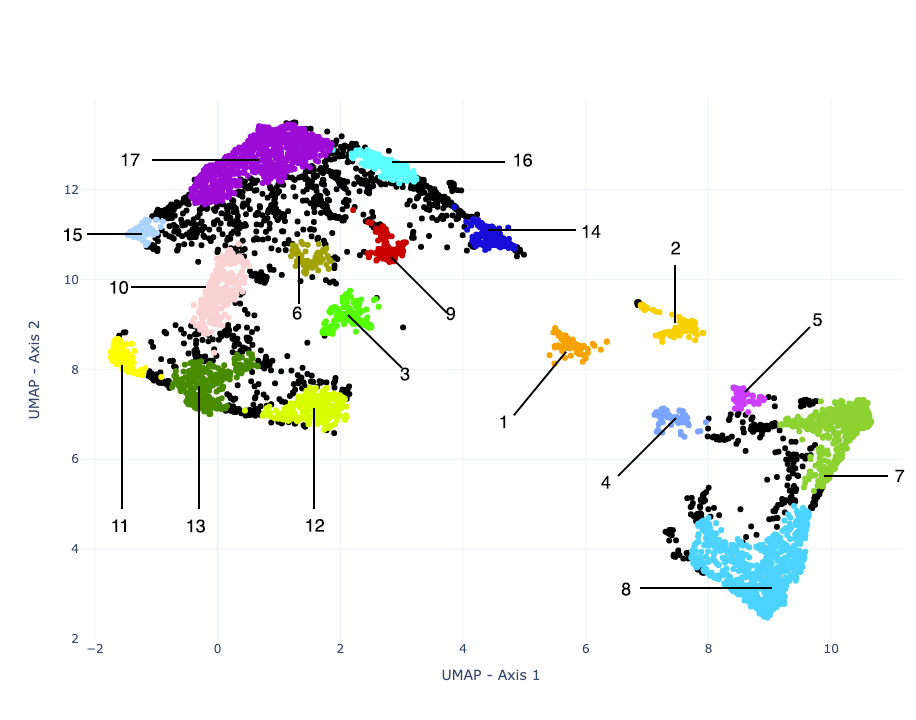
\includegraphics{03-Chapitre2/figures/fig1.png}
\caption[Two-dimensional \emph{UMAP} embedding of the benthic cover data
of the 6,554 \emph{RLS} transects.]{\footnotesize Two-dimensional \emph{UMAP} embedding of the benthic cover data
of the 6,554 \emph{RLS} transects. Each point corresponds to an \emph{RLS}
transect, coloured according to membership for the selected
\emph{UMAP-HDBSCAN} pipeline. Black dots represent points classified as
noise (n=1464). The 17 clusters can be interpreted as follows (see
Fig.~\ref{fig:chap2fig2} and S20-36): 1. \emph{Foliose brown algae}
(n=148) 2. \emph{Filamentous algae} (n=208) 3. \emph{Other Sessile
invertebrates} (n=185) 4. \emph{Foliose red algae} (n=123) 5.
\emph{Seagrass} (n=83) 6. \emph{Soft coral and gorgonians} (n=98) 7.
\emph{Bushy fucoids} (n=577) 8. \emph{Canopy forming algae} (n=894) 9.
\emph{Unconsolidated substrate} (n=151) 10. \emph{Crustose coralline and
turf algae} (n=286) 11. \emph{Green calcified algae} (n=166) 12.
\emph{Bare substrates} (n=329) 13. \emph{Crustose coralline algae}
(n=409) 14. \emph{Sand} (n=220) 15. \emph{Branching coral} (n=110) 16.
\emph{Turf and sand} (n=207) 17. \emph{Turf algae}
(n=897)}\label{fig:chap2fig1}
}
\end{figure}

\clearpage

The 17 clusters identified can be summarised hereafter according to four
broad groups (Fig.~\ref{fig:chap2fig3}, \ref{fig:chap2fig3}, see Fig S2-S19 for their
distribution on the globe and S20-36 for their interpretation with
\emph{SHAP} framework in Supporting Informations): (1) temperate
habitats, (2) subtropical and tropical habitats, (3) broadly-distributed
habitats and (4) opportunistic habitats (i.e.~habitats with documented
ecological dysfunctions - and therefore often habitats under strong
anthropogenic influence, characterised by the presence of filamentous
algal species or turf).

Transects within temperate regions can be classified according to five
major clusters associated with contrasted dominance of sessile
invertebrates, foliose red algae, seagrass, bushy foliose algae and
canopy-forming algae, as follows: cluster 3 is dominated by at least
30\% and on average 42\% of sessile invertebrates. Cluster 4 is
dominated by at least 40\% coverage of foliose red algae. Cluster 5 is
dominated by at least 30\% and on average 40\% seagrass. Cluster 7 is
dominated by at least 20\% coverage and an average of 56\% fucoid bushy
algae and an absence of canopy forming algae. Cluster 8 is characterised
by a cover of at least 20\% and an average of 55\% of canopy forming
algae with an absence of fucoid bushy algae.

Three clusters correspond to tropical and sub-tropical habitat types.
Cluster 6 which is characterised by at least 30\% and on average 37\% of
soft corals and gorgonians. Cluster 11 is composed of 20\% coverage and
an average of 35\% green calcified algae. Finally cluster 15 is composed
of at least 35\% and on average 55\% branching coral. Interestingly,
this is the only group of corals identified in the dataset given the
four categories of colony-forming corals.

Five clusters correspond to broadly-distributed habitats that can occur
across both temperate and tropical latitudes. Cluster 1 is dominated by
at least 30\% and on average 46\% brown foliose algae. Cluster 9 is
dominated by the presence of at least 30\% and on average 41\%
unconsolidated substrate. Cluster 12 has at least 30\% and on average
42\% bare substrate. Cluster 13 is characterised by 40\% and on average
51\% of crustose coralline algae with an absence of turf algae. Cluster
14 has at least 30\% and an average of 53\% sand without turf algae.

Finally, four clusters correspond to opportunistic habitats. Cluster 2
is in that respect dominated by at least 30\% coverage and an average of
39\% filamentous algae. Clusters 10, 11 and 17 are all dominated by turf
algae. Cluster 10 is composed of at least 30\% and on average 39\% of
turf algae and at least 20\% and on average 28\% of crustose coralline
algae. Cluster 16 is characterised by the presence of at least 30\% and
on average 48\% turf algae and a minimum coverage of 20\% and on average
26\% sand. Cluster 17 is composed of at least 40\% and on average 60\%
turf algae with an absence of crustose coralline.

\begin{figure}
\hypertarget{fig:chap2fig2}{%
\centering
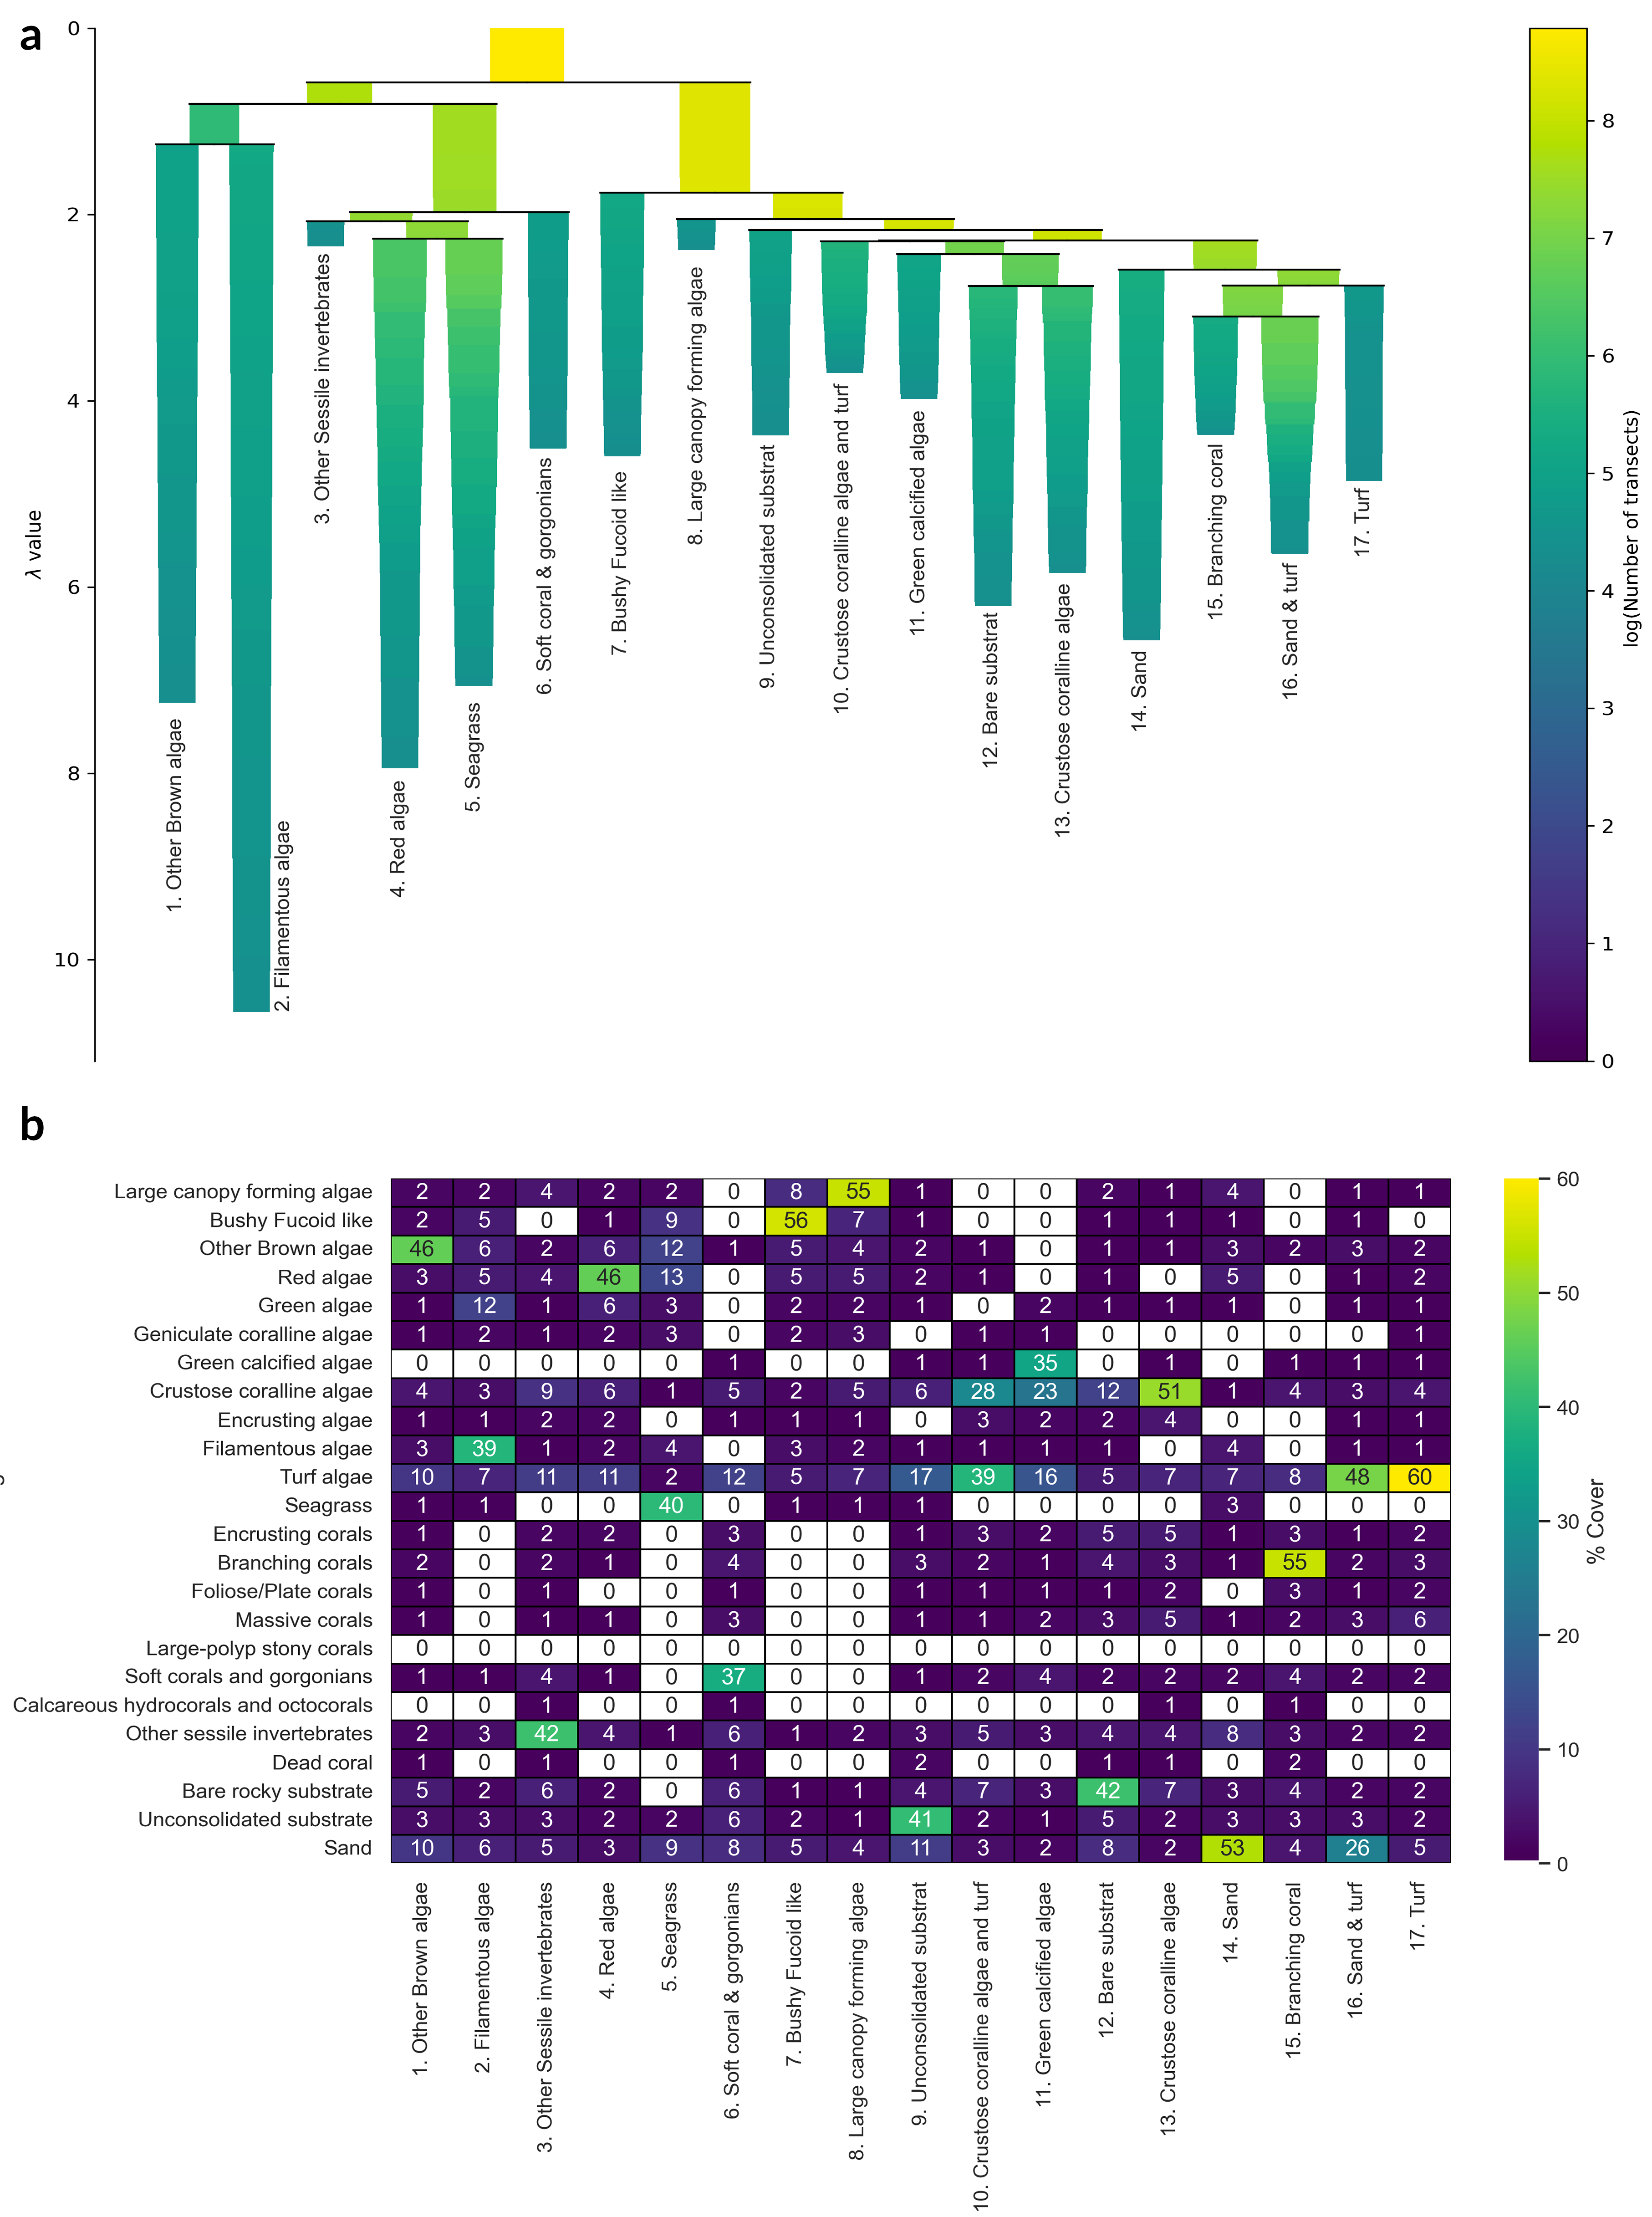
\includegraphics{03-Chapitre2/figures/fig2.png}
\caption[a. \emph{HDBSCAN} condensed clustering tree of the \emph{UMAP}
2D embedding b. Heatmap of the mean substrate coverage for each cluster identified 
by the \emph{UMAP-HDBSCAN} pipeline.]{a. \emph{HDBSCAN} condensed clustering tree of the \emph{UMAP}
2D embedding b. Heatmap of the mean substrate coverage (rounded to the
nearest integer) for each cluster identified by the \emph{UMAP-HDBSCAN}
pipeline.}\label{fig:chap2fig2}
}
\end{figure}

The clusters identified by the \emph{UMAP-HDBSCAN} pipeline show a
marked latitudinal gradient (Fig.~\ref{fig:chap2fig3}). \emph{Red
algae}, \emph{filamentous algae}, \emph{fucoids}, \emph{canopy-forming
algae} and \emph{seagrass} are essentially distributed overall in the
temperate zones across latitudes higher than 25°
(Fig.~\ref{fig:chap2fig3}). Conversely, 4 habitat states, namely
\emph{soft corals and gorgonians}, \emph{green calcified algae},
\emph{sand and turf} and \emph{branching coral} essentially occur in
tropical latitudes (lower than 25°) (Fig.~\ref{fig:chap2fig3}). However,
some groups are relatively ubiquitous across all surveyed latitudes such
as those associated with transects classified as \emph{noise},
\emph{bare} and \emph{unconsolidated substrate}, \emph{brown algae},
\emph{crustose coralline algae} with and without \emph{turf algae} and
\emph{turf algae} (Fig.~\ref{fig:chap2fig3}).

\begin{figure}
\hypertarget{fig:chap2fig3}{%
\centering
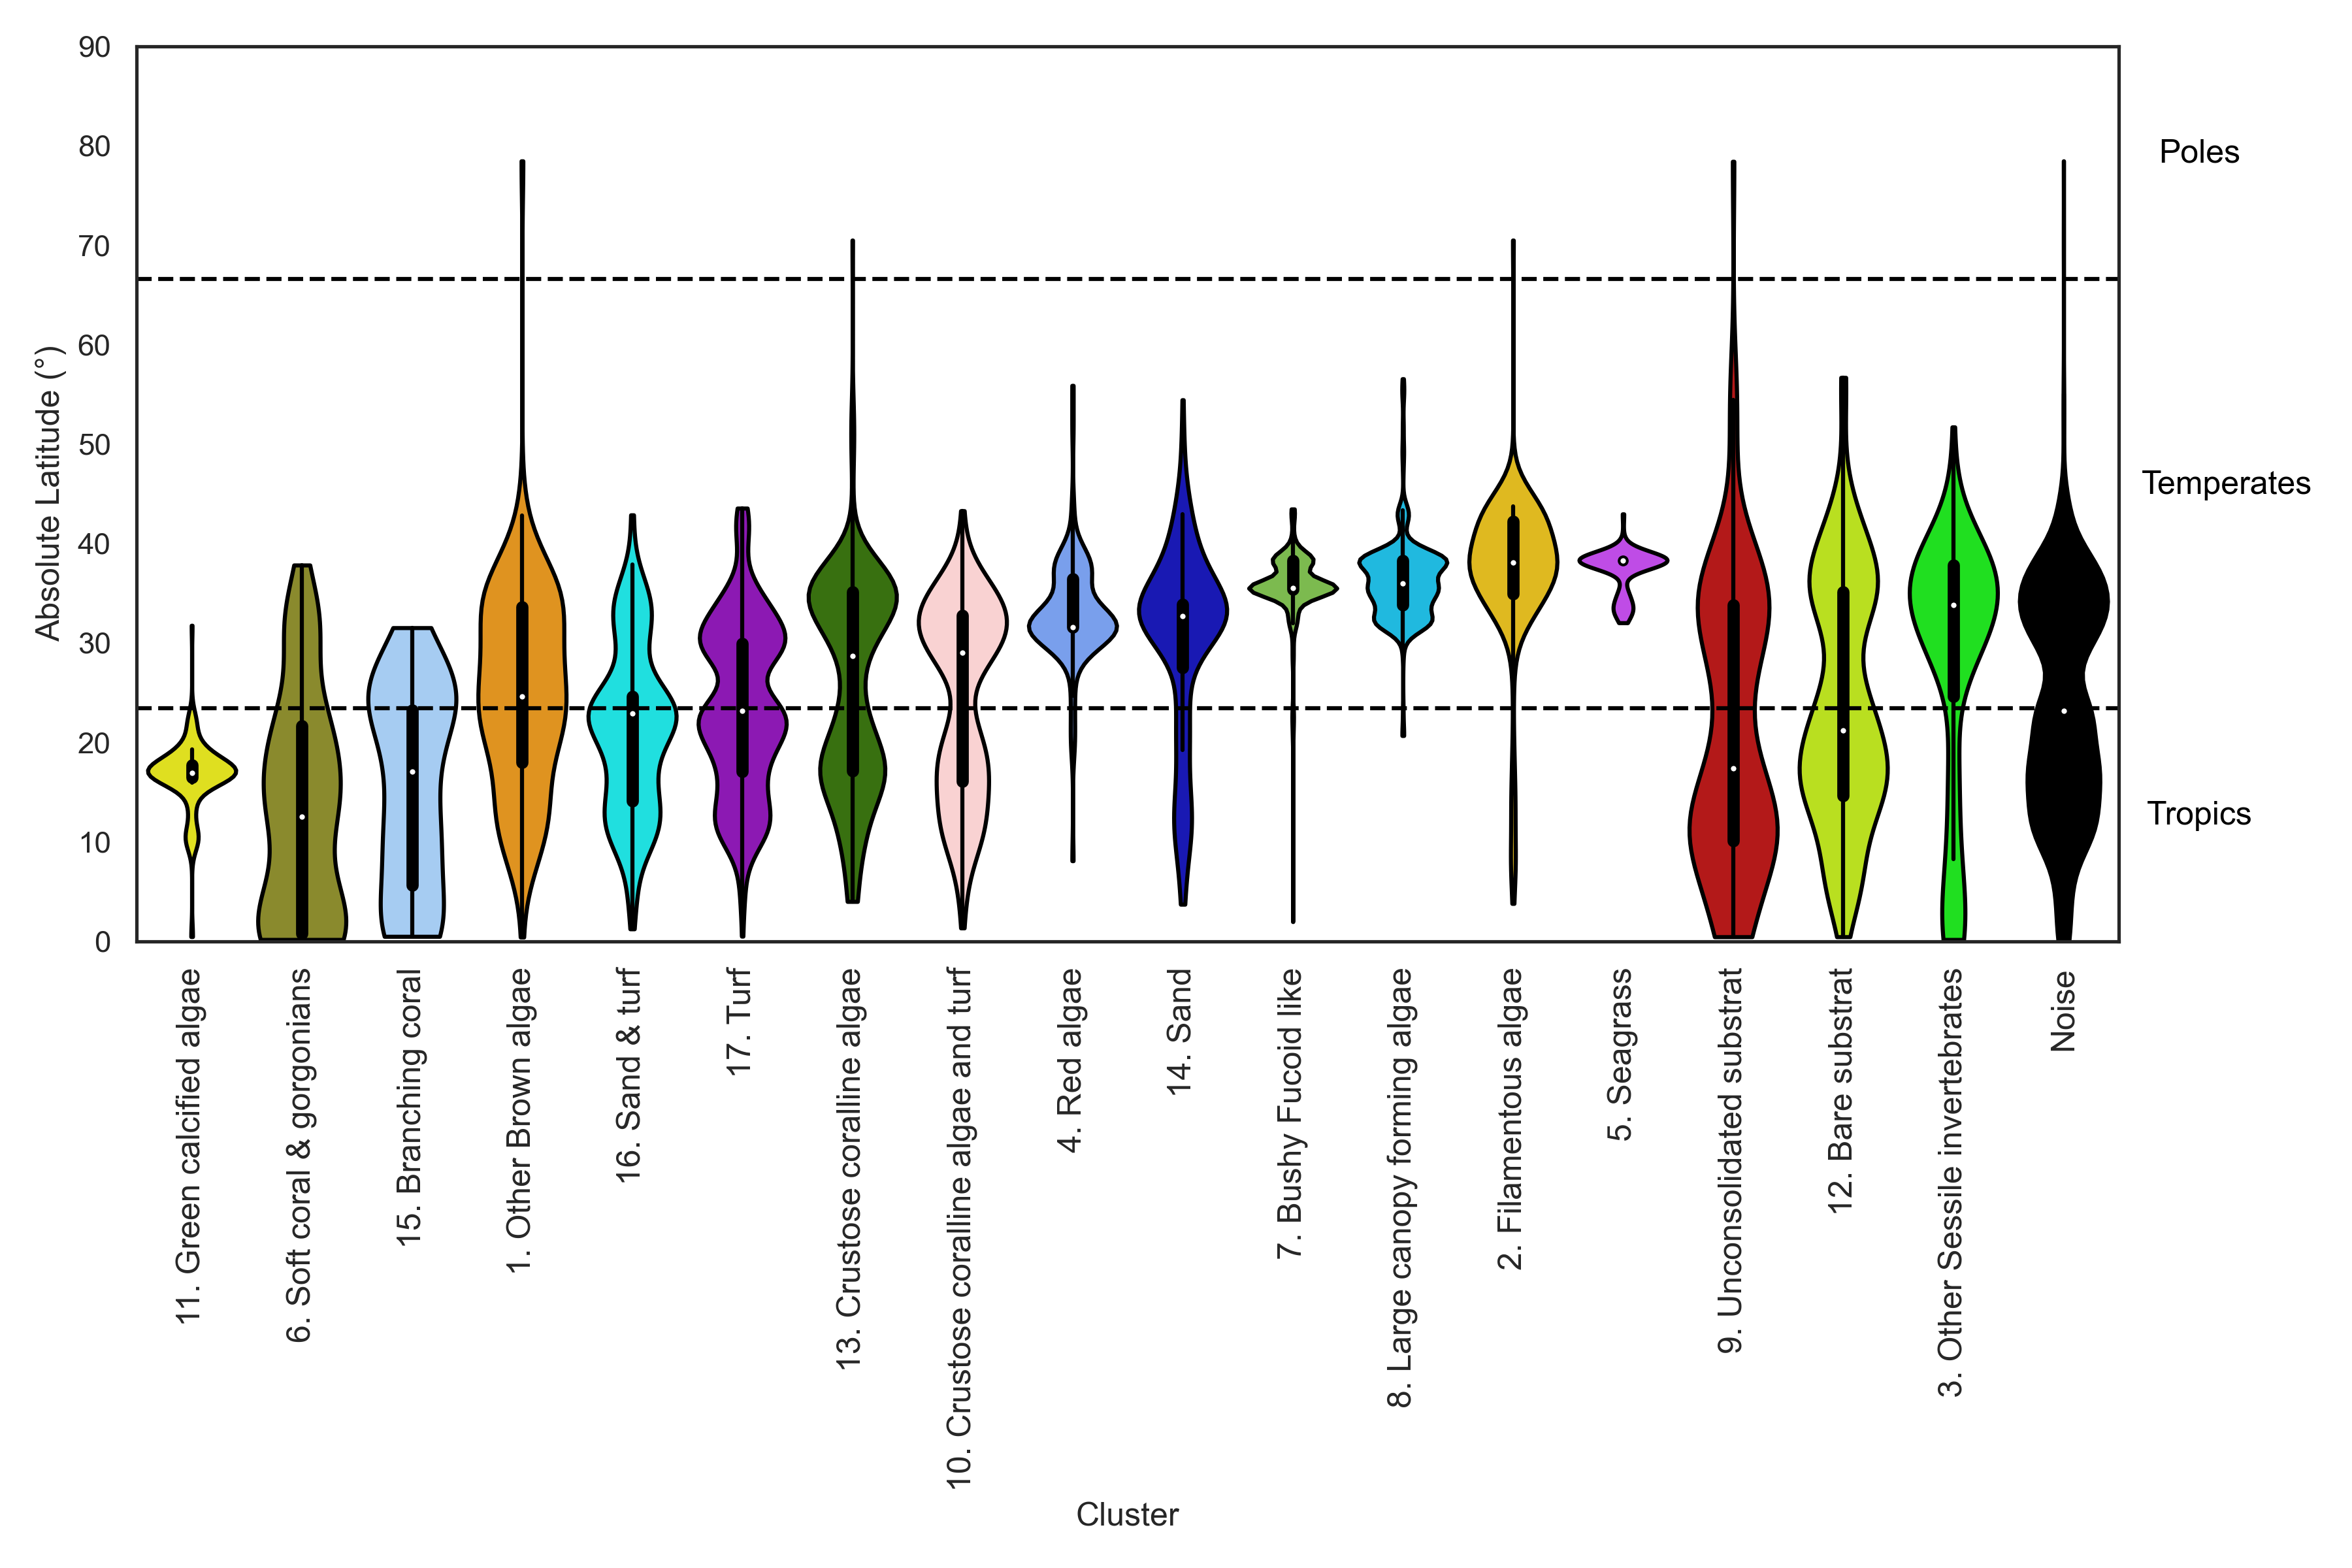
\includegraphics{03-Chapitre2/figures/fig3a.png}
\caption{Violin plot of the absolute latitudinal distribution of the
different hard cluster solutions.}\label{fig:chap2fig3}
}
\end{figure}

The spatial distribution of transects sampled by \emph{RLS} volunteers
is particularly concentrated in Australia (Fig.~\ref{fig:chap2fig4} a).
However, other areas such as the Caribbean, the Azores, and French
Polynesia have also been extensively surveyed with more than 50
transects (Fig.~\ref{fig:chap2fig4} a). Globally, three habitat types
dominate in terms of occurrences across all surveyed ecoregions, namely
\emph{bare substrate} (n = 20), \emph{turf} (n = 17), and
\emph{canopy-forming algae} (n = 11). These three habitat types dominate
in 37\% of the ecoregions sampled by the \emph{RLS}
(Fig.~\ref{fig:chap2fig4} b). Two habitat types identified by the
\emph{UMAP-HDBSCAN} pipeline, \emph{seagrass} and \emph{red algae}, are
not dominant in any of the world's ecoregions. The patterns of dominance
of the different clusters also vary along the latitudinal gradient
(Fig.~\ref{fig:chap2fig4} b), in line with the latitudinal distribution
of each cluster (Fig.~\ref{fig:chap2fig3}). These latitudinal variations
of dominance are visible both at a global scale, but also along certain
regions. For instance, a decrease in prevalence of sites in the
canopy-forming algae cluster accompanies an increase in sites in the
turf cluster along the coastline from southern to northern Australia
(Fig.~\ref{fig:chap2fig4} b).

The proportion of noisy transects is highly heterogeneous across the
globe (Fig.~\ref{fig:chap2fig4} c). Noisy transects represent 23\% of
all transects analysed, but are present in some areas more than in
others. For example, in the Southern California Bight (western USA),
Bight of Sofala/Swamp Coast (Eastern Africa), the Seychelles, and in
Three Kings-North Cape (northern New Zealand), at least 60\% of
transects are classified as noisy (Fig.~\ref{fig:chap2fig4} c). While
these four ecoregions share in common a low number of transects sampled
(Fig.~\ref{fig:chap2fig4} a), no significant correlation was found
between the proportion of transects classified as noisy and the number
of transects done in each ecoregion
(\(\tau_{Kendall} = 0.05 \text{, p}= 0.54\); Fig. S37 Supporting
Information). Moreover, 12 ecoregions sampled out of the 83 by the
\emph{RLS} had no transects that were classified as noisy
(Fig.~\ref{fig:chap2fig4} c).

Areas with the highest diversity of habitat types, based on both the
number of clusters occurring and on their relative proportions in the
ecoregions, are concentrated in eastern and western Australia, as well
as in the Caribbean and the Tuamotus (Fig.~\ref{fig:chap2fig4} d). Areas
with the lowest Gini-Simpson values are the Southern California Bight
(western USA) and Bight of Sofala/Swamp (eastern Africa) Coast with a
Gini index of 0 (Fig.~\ref{fig:chap2fig4} d). It should be noted,
nevertheless, that there is a weak correlation between the Gini-Simpson
index and the number of transects carried out in the ecoregion
(\(\tau_{Kendall} = 0.29 \text{, p} < 0.001\); Fig. S38 in Supporting
Information).

\begin{figure}
\hypertarget{fig:chap2fig4}{%
\centering
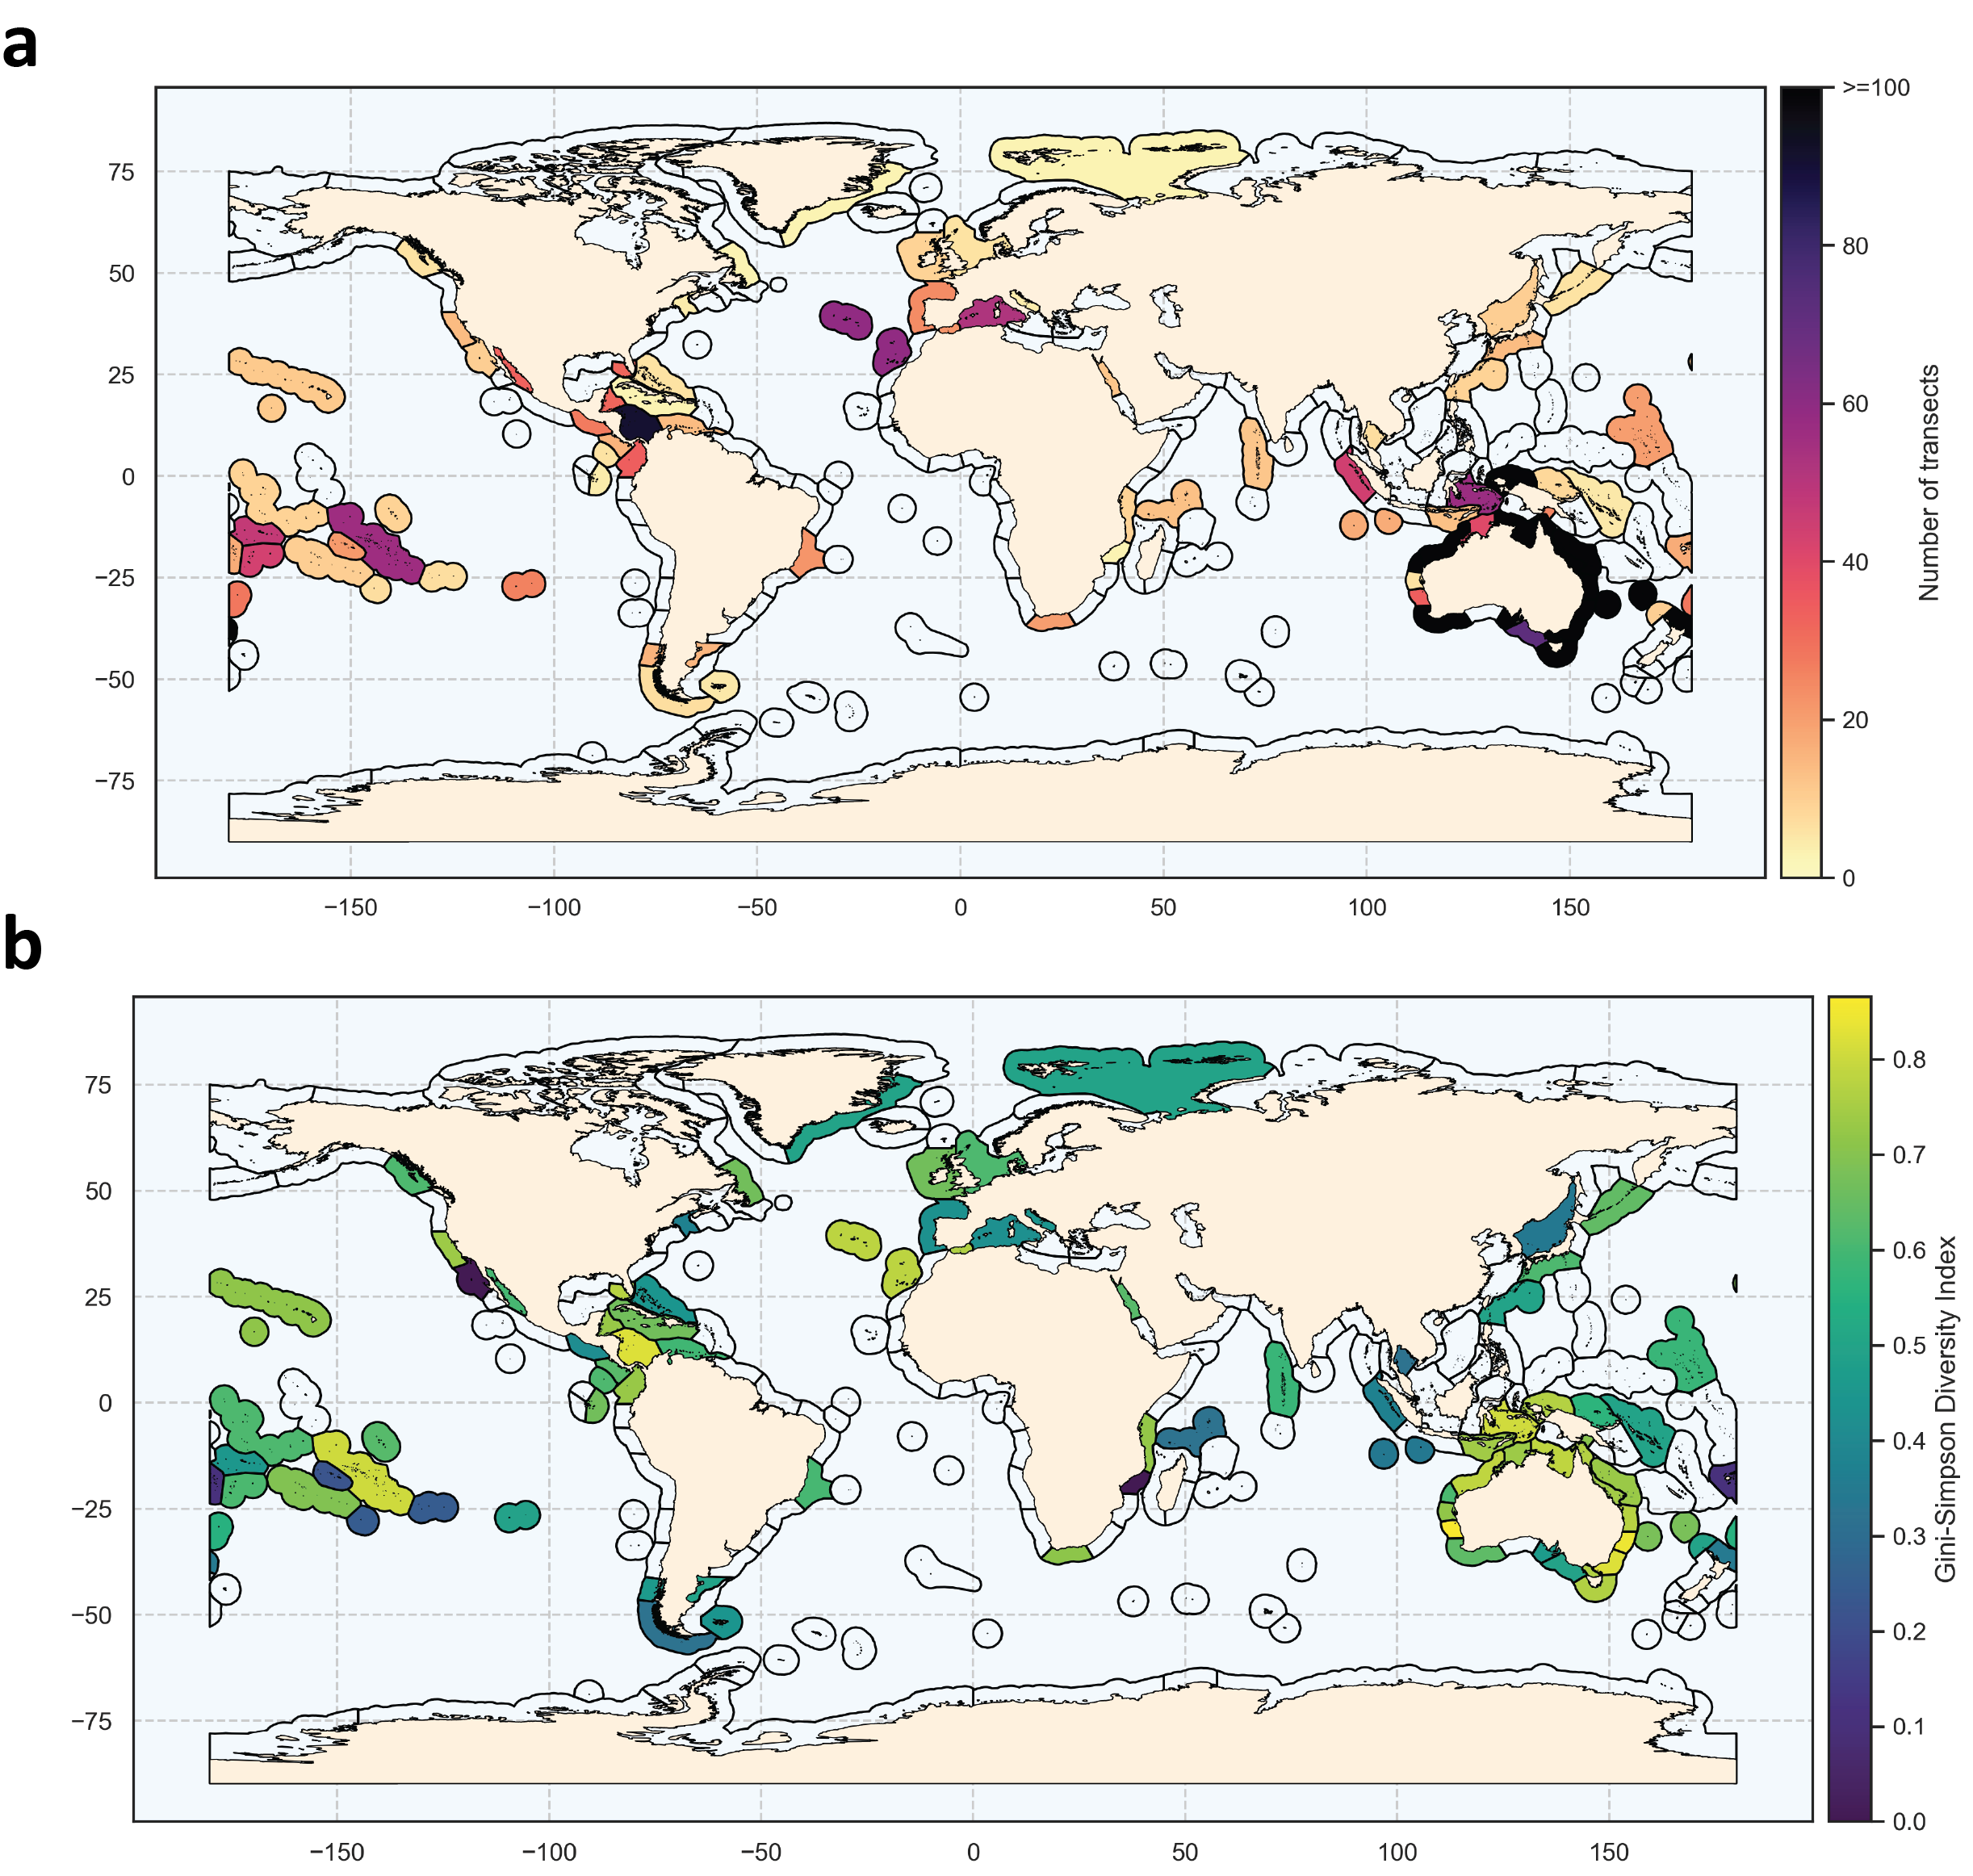
\includegraphics{03-Chapitre2/figures/fig4_ab.png}
\caption{a. Spatial distribution of reef surveys from the Reef Life
Survey database used for analyses. b. Map of dominant clusters in each
MEOW ecoregion. Dominant clusters were determined as the greatest count
of transect labels in each ecoregion. c.~Spatial distribution of the
proportion of transects classified as noise in each ecoregion.
d.~Gini-Simpson diversity index calculated by the occurrence of clusters
in each ecoregion of the world.}\label{fig:chap2fig4}
}
\end{figure}
\begin{figure}
\ContinuedFloat
\centering
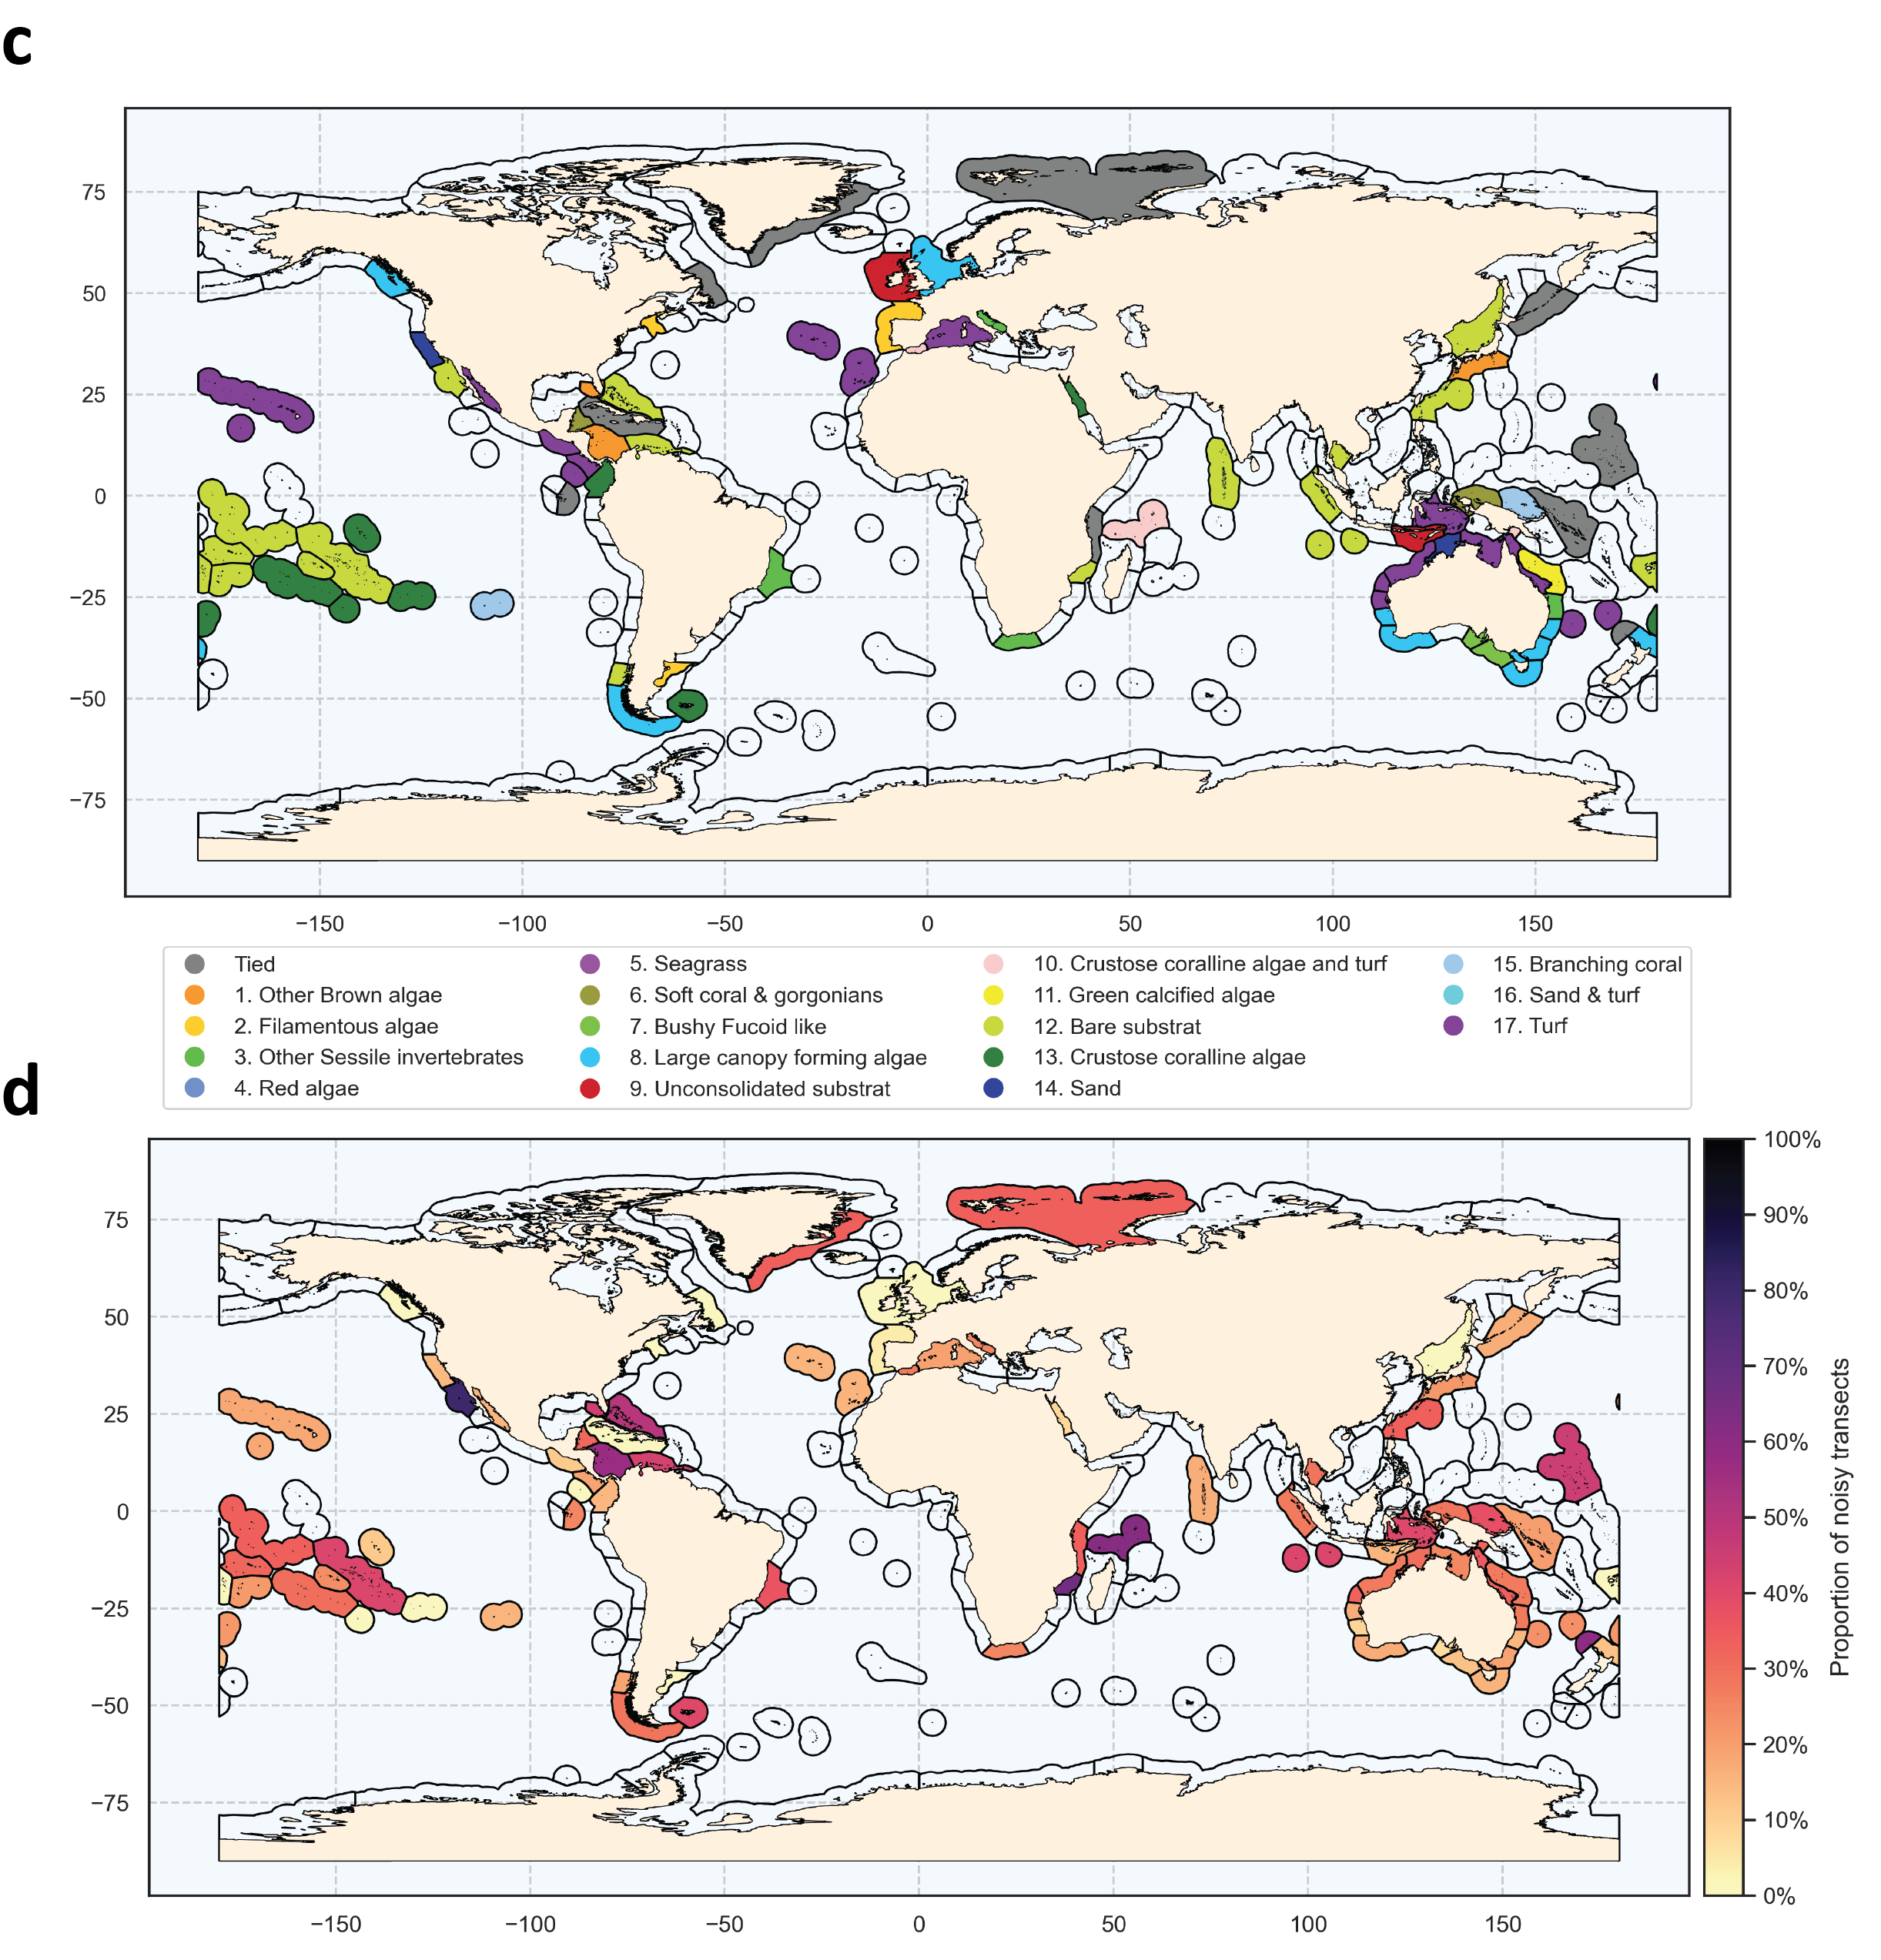
\includegraphics{03-Chapitre2/figures/fig4_cd.png}
\caption[]{a. Spatial distribution of reef surveys from the Reef Life
Survey database used for analyses. b. Map of dominant clusters in each
MEOW ecoregion. Dominant clusters were determined as the greatest count
of transect labels in each ecoregion. c.~Spatial distribution of the
proportion of transects classified as noise in each ecoregion.
d.~Gini-Simpson diversity index calculated by the occurrence of clusters
in each ecoregion of the world.}
\end{figure}

At a finer spatial scale, it is also possible to identify spatial and
temporal transitions in the occurrence of the different clusters
(Fig.~\ref{fig:chap2fig5}). Along spatial gradients, clusters classified
as noise may be a sign of the presence of an ecotone, as in the Cape
Howe region in southeastern Australia (Fig.~\ref{fig:chap2fig5} b).
These transects classified as noise separate an area with transects
classified as bare substrate/crustose coralline algae to the north from
an area to the south with transects classified as canopy forming algae
and red algae (Fig.~\ref{fig:chap2fig5} b).

\begin{figure}
\hypertarget{fig:chap2fig5}{%
\centering
\includegraphics{03-Chapitre2/figures/fig5.png}
\caption[Well-sampled ecoregions in Australia, with high number of
transects and temporal replications between 2008 and 2021.]{Well-sampled ecoregions in Australia, with high number of
transects and temporal replications between 2008 and 2021. b.
Distribution of 44 sites surveyed between 2008 and 2021 in the Cape Howe
region; Colour coding indicates cluster identity. Dots are jittered
along the y-axis. c.~Number and proportion of transects in the different
clusters for the period 2008-2013 in the four ecoregions highlighted in
a. d.~The same analysis for the period 2014-2021.}\label{fig:chap2fig5}
}
\end{figure}

The relative proportion of the different clusters is overall stable
overtime when comparing the early and the late 2010s. In this temperate
zone, the most predominant cluster remains the canopy forming algae,
followed by transects classified as noise (Fig.~\ref{fig:chap2fig5} c).
Noticeable changes between the two periods include: the proportion of
transects classified as sand decreased from 10\% to below 8\%, while the
proportion of transects classified as \emph{turf} increased from 7\% to
exceed 10\% (Fig.~\ref{fig:chap2fig5} c \& d). Transects classified as
\emph{turf} or \emph{crustose coralline and turf} or \emph{sand and
turf}, represented approximately 16\% of the clusters between 2008-2013
and increased to nearly 19\% for the period 2015-2021. The proportion of
transects classified as bare substrate declined from approximately 5\%
in 2008-2013 to only 1\% of the transects in 2015-2021.

\clearpage

\hypertarget{discussion-chapt2}{%
\section{Discussion}\label{discussion-chapt2}}

The \emph{UMAP-HDBSCAN} clustering pipeline identified 17 distinct
clusters within all the \emph{RLS} transects performed globally across a
range of coastal temperate and tropical regions. Within these groups, we
found different biogenic habitats whose distribution patterns match with
current biogeographic knowledge of benthic ecosystems: for example,
\emph{bushy fucoid-like algae}, and \emph{canopy-forming algae}
predominantly occur in temperate waters \autocites[
]{Assis_2020}{Jayathilake_2020}, while \emph{soft corals and
gorgonians}, and \emph{branching coral} are more frequent in tropical
waters \autocites[ ]{Jones_2019}{Wirabuana_2019}. Our analysis also
highlights habitat types that occur across the globe, including (1)
different granulometric facies like \emph{sand}, \emph{unconsolidated
substrate}, and \emph{bare substrate,} as well as (2) different habitat
types dominated by low-profile algae , such as \emph{crustose coralline
algae} or \emph{turf algae}. The latter are known to occur across the
globe and can dominate benthic substrates in diverse conditions
\autocites[ ]{Connell_2014}{Liu_2018}.

In addition, this classification also distinguishes between different
ecological states of these habitats (hereafter refers to as ``habitat
state''), including known alternative successional stages, or different
degradation states of these habitats (Fig.~\ref{fig:chap2fig6}). For
example, the clusters \emph{crustose coralline algae}, \emph{crustose
coralline algae and turf} and \emph{turf} provide an interesting
template to describe the habitat transitions described in
\textcite{Cornwall_2023}, which suggests that a shift from
\emph{crustose coralline algae} to \emph{turf} domination reduces reef
carbonate production. Similarly, the clusters \emph{branching coral},
\emph{turf and sand} and \emph{turf} can be used to describe and
quantify in a standardised manner the transitions between corals and
turf dominated habitats that are occurring more frequently due to
anthropogenic pressures \autocite{Jouffray_2015}.
Fig.~\ref{fig:chap2fig5} b also illustrates the occurrence along the
southeastern Australian coastline of alternative ecological states on
temperate reefs, where dense macroalgal canopies dominated by
\emph{Ecklonia radiata} (here \emph{large canopy-forming algae}), can
shift to extensive barrens (here \emph{bare substrate} or \emph{crustose
coralline algae}) following destructive grazing by the long-spined sea
urchin \emph{Centrostephanus rodgersii} \autocite{Ling_2009}. Thus, our
approach can classify reef cover data collected across the globe with
the \emph{RLS} protocol into an ecologically sound template to explore
common reef habitat transitions under anthropogenic pressures
\autocite{Donovan_2018}.

\begin{figure}
\hypertarget{fig:chap2fig6}{%
\centering
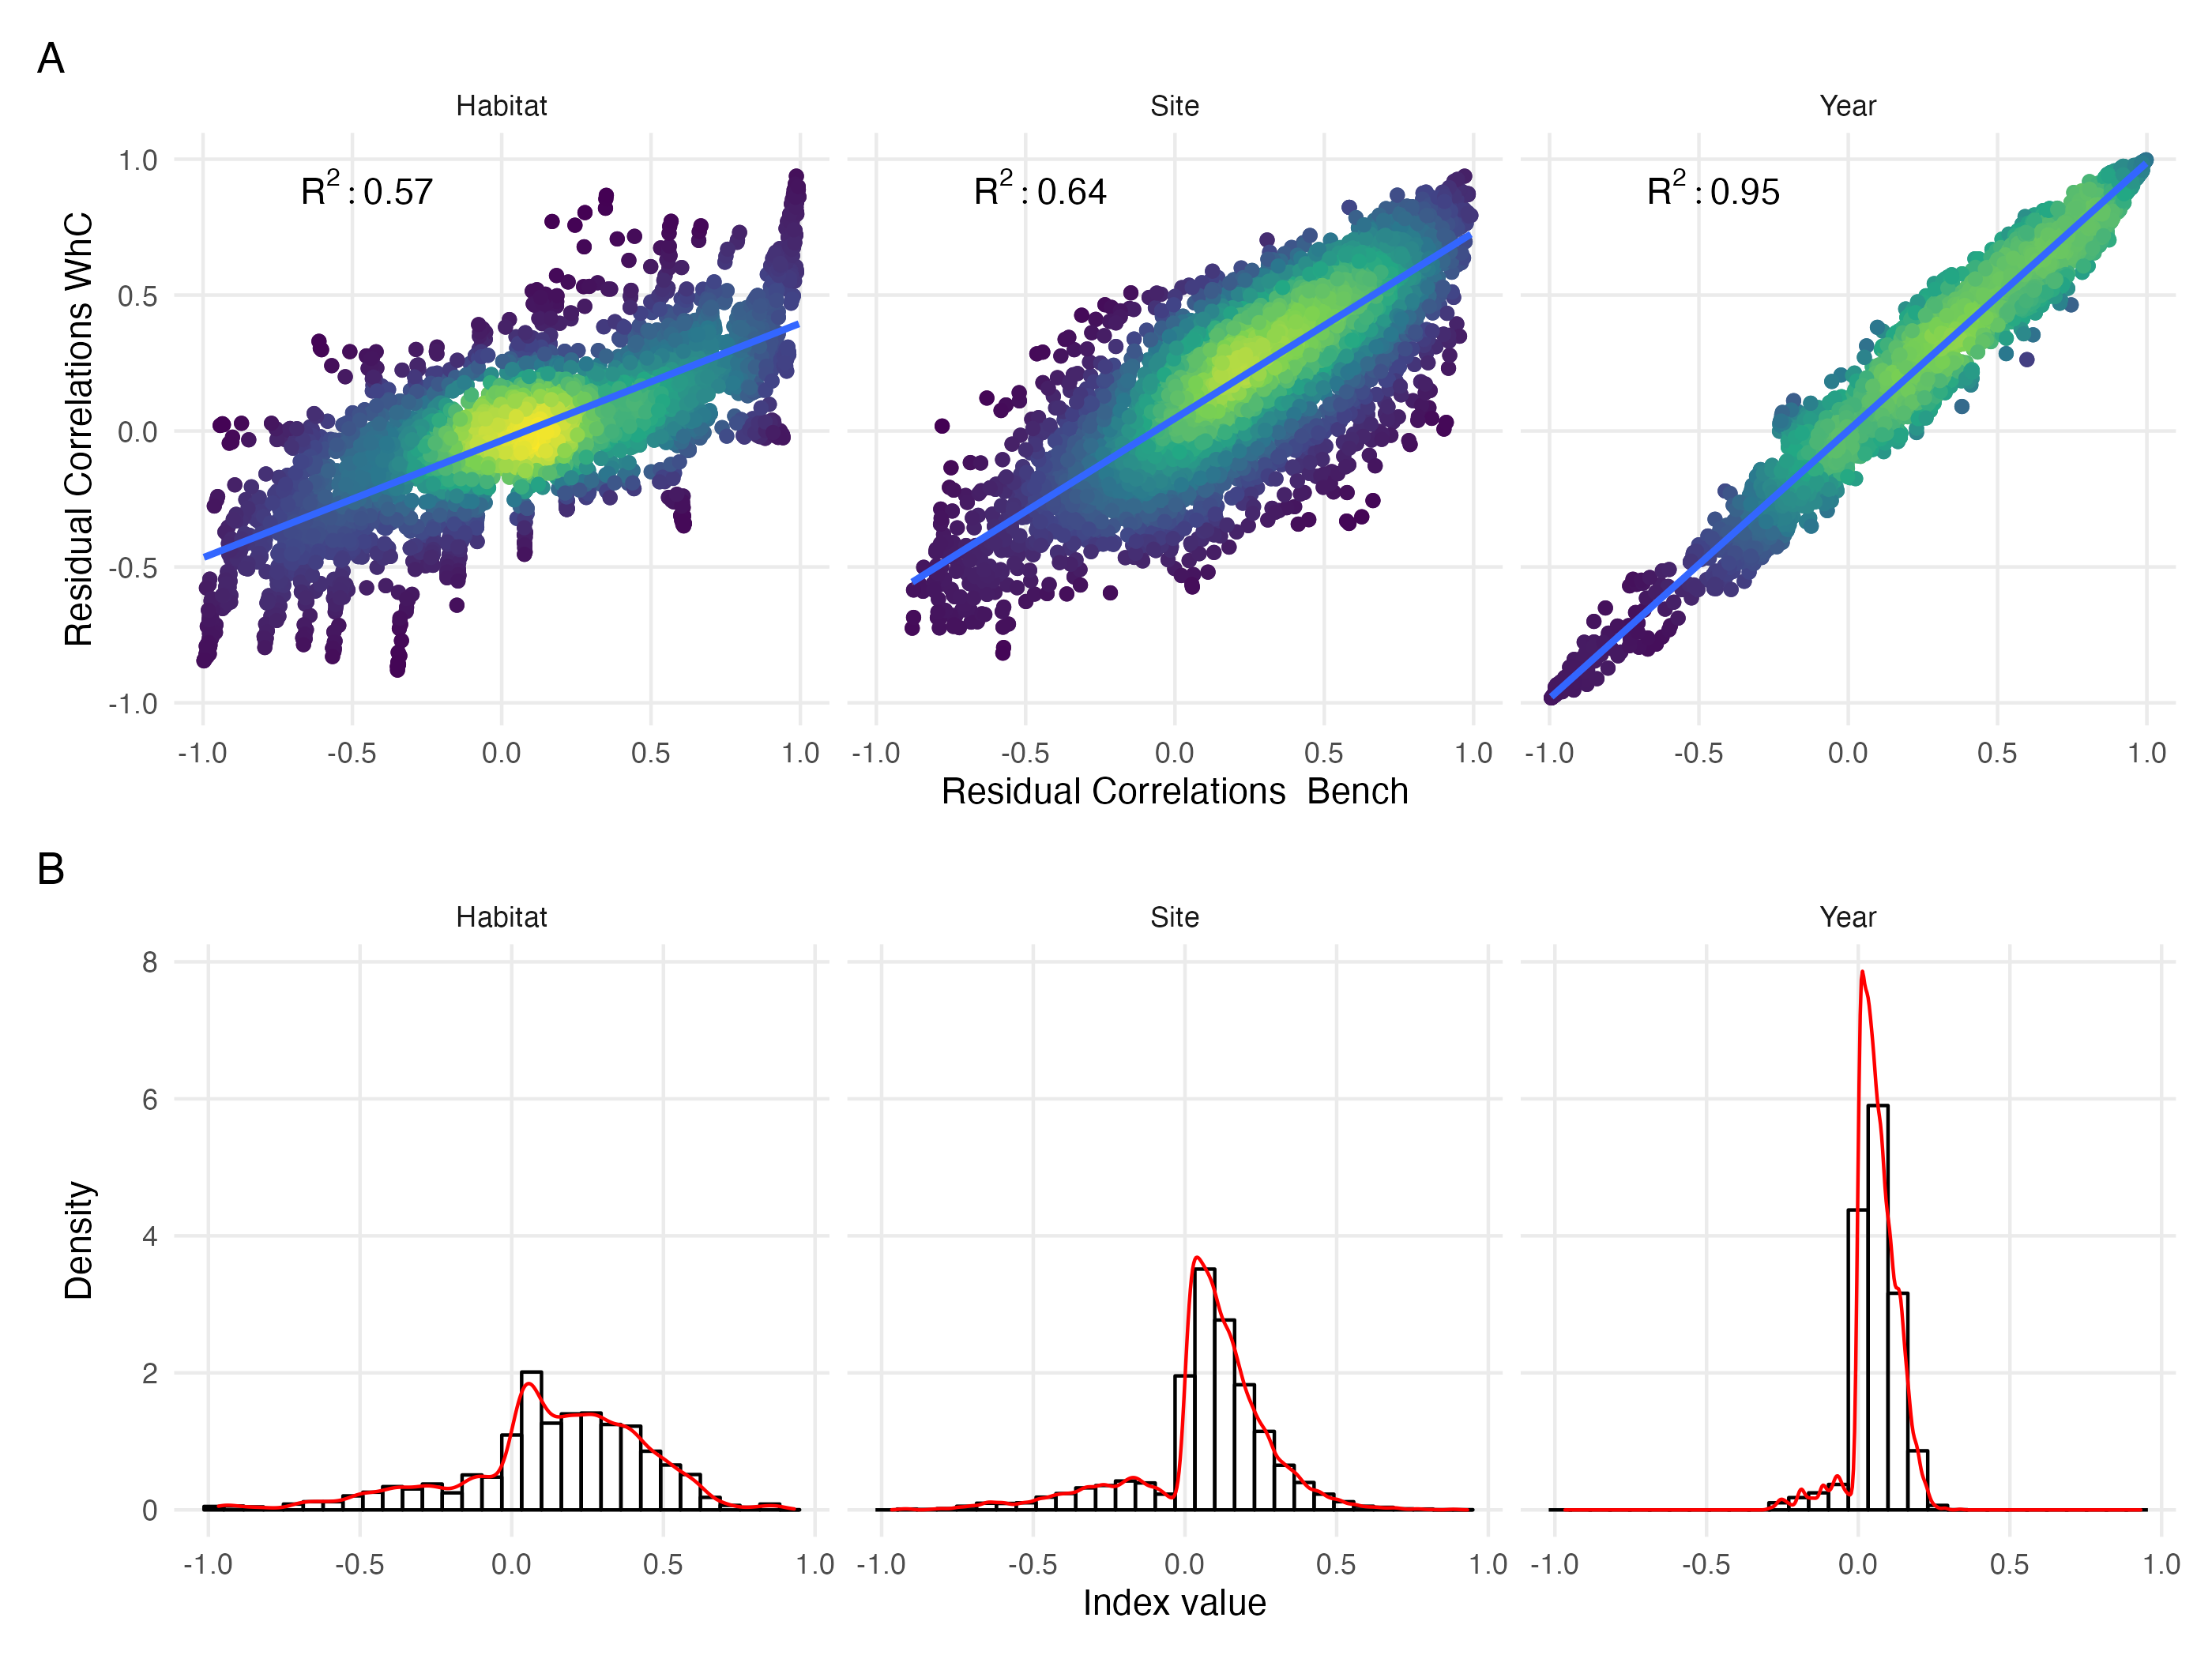
\includegraphics{03-Chapitre2/figures/fig6.png}
\caption[Two-dimensional UMAP embedding of the 5,090 clustered
\emph{RLS} transects.]{Two-dimensional UMAP embedding of the 5,090 clustered
\emph{RLS} transects. Each picture is representative of its cluster. The
arrows indicate potential transitions as identified in
\textcite{Jouffray_2015} and
\textcite{Cornwall_2023}.}\label{fig:chap2fig6}
}
\end{figure}

Certain of the habitat states identified here on the global \emph{RLS}
dataset match well with the habitat states previously identified by
\textcite{Cresswell_2017}, who applied another clustering approach to an
Australian subset of the \emph{RLS} dataset. In particular, some of our
groups (i.e.~\emph{canopy forming algae}, \emph{turf algae},
\emph{filamentous algae} and \emph{branching coral}), match well with
four out of the nine habitat states identified by
\textcite{Cresswell_2017} (i.e.~''Canopy algae'', ``Turf'', ``Epiphytic
filamentous algae--caulerpa'' and ``Coral''; see Table 1 in
\textcite{Cresswell_2017} for a detailed description of their habitat
states and Fig.~\ref{fig:chap2fig2} b in this paper for comparison).
Furthermore, we identified more finely-resolved habitat states here
relative to the classification proposed by \textcite{Cresswell_2017}.
The clusters \emph{crustose coralline algae} and \emph{bare substrate}
identified here are amalgamated into a single ``Barren'' cluster in
\textcite{Cresswell_2017}, while the clusters \emph{red algae} and
\emph{other brown algae} further detail what \textcite{Cresswell_2017}
identified as one single ``Foliose algae'' group. Thus, our large-scale
spatial approach overall confirms the habitat types defined by
\textcite{Cresswell_2017} while to some extent providing a more nuanced
distinction between similar habitats. Nevertheless, our analysis only
managed to capture one type of coral reef, contrary to what we might
have expected, but there may be several reasons for this result. The
proportion of coral cover within coral reefs exhibits significant
variability, as indicated by \autocite{Death_2012}, although multiple
sub-categories of coral have been merged together to circumvent this
issue (see Appendix A Table S1). Additionally, the morphological
diversity of these reefs is extensive, with variations in surface areas
\autocite{Zawada_2019}. Such variability might elucidate why a singular
group of corals, \emph{Branching coral} is found as a group, since some
species of \emph{Acropora spp.} are able to establish colonies with
expansive surface areas. Hence, our data-driven approach yields a finely
resolved classification that comprises typical benthic habitats
(e.g.~seagrass meadows, coral reefs, kelp forests) that are common
across all major seafloor habitat classification scheme
(e.g.~\emph{European Nature Information System};
\textcite{Bajjouk_2015}).

Our global classification of the \emph{RLS} data highlights hotspots of
diversity in terms of benthic habitats and habitat states. Four
ecoregions in particular, the Eastern (Manning-Hawkesbury ecoregion) and
Western Australia (Houtman ecoregion), the Caribbean, and the Tuamotus
Archipelago, showed a high diversity of habitat types (considering both
richness and evenness). The high diversity of habitat types we report in
the Caribbean and in the Tuamotus Archipelago potentially contribute to
explain the high marine diversity of reef fishes reported in these
tropical coral reefs, despite their small area at a global scale
\autocite{Cowman_2017}. In the transition zones between temperate and
tropical waters, such as the Manning-Hawkesbury or the Houtman
ecoregions in eastern and western Australia respectively, the high
diversity of benthic habitat types we observe could be explained by a
high diversity of foundation species. Indeed, high biodiversity is
typical of transitional environmental conditions where ecological
niches, which are overall disjointed, overlap \autocite{Ferro_2014}.
This phenomenon is well known for multiple taxon such as birds
\autocite{Altamirano_2020}, plants \autocite{Lemessa_2023} or reef fish
\autocite{Pinheiro_2018} and also seems to apply to a certain extent to
biogenic habitats like coralline red algae \autocite{Sissini_2022}. Such
subtropical or warm temperate zones are also identified as regions where
both mobile fauna \autocite{Verges_2014} or sessile habitat-forming
species assemblages \autocite{Marzloff_2018} are likely to undergo
tropicalisation, which implies that native temperate assemblages can
co-occur with warmer species assemblages undergoing poleward
climate-driven range shifts. Our finely resolved classification could be
modelled against environmental predictors in future work to understand
and predict the state of benthic habitats under current and future
conditions (e.g. \textcite{Belanger_2012}).

Beyond exploring spatial patterns of benthic biodiversity, our
classification of the \emph{RLS} dataset offers a new perspective to
explore temporal changes in benthic habitat states. Within the most
resampled ecoregions (essentially located in southeastern Australia), we
quantified temporal changes in the occurrence of certain habitat types
between the period 2008-2013 and 2014-2021. For example, the proportion
of transects classified as \emph{large canopy-forming algae} shows an
increase in the Manning-Hawkesbury ecoregion (Fig. S39 in Supplementary
Informations) while it decreased in the Cape Howe ecoregion (Fig. S40 in
Supplementary Informations). These regional differences can be explained
by local changes in the environment \autocite{Krumhansl_2016}. We also
observe an increase in transects classified as \emph{turf algae} among
the five ressampled ecoregions (e.g.~+67\% increase between the two
periods), in line with findings of an increase in turf algae due to both
global climate change and local anthropogenic impacts
\autocite{Filbee-Dexter_2018}. Note, however, that temporal analysis of
changes was restricted to only 5 southeastern Australian data-rich
ecoregions out of a total of 232 worldwide. This reflects the strong
geographical bias of the \emph{RLS} dataset, with 78\% of transects
performed along Australian shores. Moreover, marginal changes in the
proportion of certain habitat states, such as \emph{red algae} or
\emph{seagrass}, may also be due to the random positioning of transects,
which does make the survey protocol accessible to citizen scientists but
does not guarantee truly replicated observations through time.

Beyond exploring spatial patterns of benthic biodiversity, our
classification of the \emph{RLS} dataset offers a new perspective to
explore temporal changes in benthic habitat states. Within the most
frequently sampled ecoregions (essentially located in southeastern
Australia), we quantified temporal changes in the occurrence of certain
habitat types between the period 2008-2013 and 2014-2021. The proportion
of transects classified as \emph{large canopy-forming algae} shows an
increase in the Manning-Hawkesbury ecoregion (Fig. S39 in Supplementary
Informations) while it decreased in the Cape Howe ecoregion (Fig. S40 in
Supplementary Informations). These regional differences can be explained
by local changes in the environment \autocite{Krumhansl_2016}, including
poleward expansion of urchin barrens \autocite{Ling_2018}. We also
observe an increase in transects classified as \emph{turf algae} among
the five ressampled ecoregions (e.g.~+67\% increase between the two
periods), in line with findings of an increase in \emph{turf algae} due
to both global climate change and local anthropogenic impacts
\autocite{Filbee-Dexter_2018}. Note, however, that temporal analysis of
changes was restricted to only 5 southeastern Australian data-rich
ecoregions out of a total of 232 worldwide. This was due to the
distribution of data availability, which is heavily focussed within the
region that \emph{RLS} originated from (southern Australia). Moreover,
marginal changes in the proportion of certain habitat states, such as
\emph{red algae} or \emph{seagrass}, may also be due to the random
positioning of transects within a site through time (as opposed to
fixed). This is beneficial for greater site replication and for
application by citizen scientists, but adds an extra source of noise to
observations within sites through time.

Overall benthic habitat changes may reflect a range of processes,
including ecological ones such as temporal variability in the cover of
habitat-forming species (e.g. \textcite{Wernberg_2016}) in relation to
climate-driven environmental changes (i.e.~tropicalisation of
tropical-temperate transition zones \autocite{Horta_2014}, marine
heatwaves \autocite{Wernberg_2016}) or to trends in human stressors (i.e
nutrients and organic pollution runoffs, impacts from coastal human
populations; \textcite{Halpern_2019}), as well as methodological ones,
such as variability in transect location or in sampling effort through
time (e.g. \textcite{Stuble_2021}). Identifying the processes driving
the observed habitat transitions could help better characterise the
impact of anthropogenic activities on benthic habitats (see for example
\textcite{Donovan_2018} for a similar approach at a finer spatial
scale). Our classification could thus provide an interesting template to
further explore changes in benthic habitats across the world
\autocite{Edgar_2023}.

Nonetheless, not all expected transitions between habitats, or
alternative ecological states, come out in the different clusters. Some
transitory states may be classified as noise if they are too scarcely
observed in the dataset to constitute a cluster of their own.
Understanding the drivers behind the transects classified as noise can
reveal valuable information about the factors influencing habitat
variability and the ecological processes driving shifts between
different states. This includes deciphering the reasons for a noise
classification, such as variations in environmental conditions, biotic
interactions, or anthropogenic disturbances. By investigating these
aspects, researchers can gain crucial insights into the dynamics and
transitions occurring between habitat states and alternative ecological
states.

The \emph{UMAP-HDBSCAN} clustering pipeline presented in this study
demonstrates remarkable robustness and versatility, leveraging global
data to identify fine-scale patterns within coastal temperate and
tropical ecosystems. Because of its hierarchical structure, this
pipeline aligns well with established classification standards and
facilitates a first data-driven description of global patterns in
habitat states, which constitutes a valuable database to explore the
influence of local and global drivers of benthic habitat states.
Additionally, the pipeline's capability to handle non-linear data and
accommodate noise underscores its adaptability to various ecological
contexts and data sources (e.g.~citizen science).

\clearpage

\printbibliography[heading=subbibintoc, title={Bibliographie}]
\end{refsection}